\documentclass{article}

\PassOptionsToPackage{numbers, compress}{natbib}

\usepackage[final]{neurips_2022}

\usepackage[utf8]{inputenc} % allow utf-8 input
% \usepackage[T1]{fontenc}  % removed: incompatible with XeLaTeX
\usepackage{hyperref}       % hyperlinks
\usepackage{url}            % simple URL typesetting
\usepackage{booktabs}       % professional-quality tables
\usepackage{amsfonts}       % blackboard math symbols
\usepackage{nicefrac}       % compact symbols for 1/2, etc.
\usepackage{microtype}      % microtypography
\usepackage{xcolor}         % colors
\usepackage{todonotes}

\usepackage{wrapfig}

\usepackage{colortbl}
\definecolor{myy}{RGB}{126,95,0}
\definecolor{mygray}{gray}{.85}
\definecolor{lightgray}{gray}{.95}
\usepackage{multirow}
\usepackage{graphicx}
\newcommand{\tabincell}[2]{\begin{tabular}{@{}#1@{}}#2\end{tabular}}
\newcommand{\myparagraph}[1]{\vspace{1pt}\noindent{\bf #1}}
\usepackage{amsmath}
\usepackage{subfigure}
\usepackage{capt-of}
\usepackage{makecell}


\title{运动Transformer：全局意图定位与局部运动精炼（Motion Transformer with Global Intention Localization and Local Movement Refinement）}


\author{
	Shaoshuai Shi,\quad
	Li Jiang,\quad
	Dengxin Dai,\quad
	Bernt Schiele\\
Max Planck Institute for Informatics, Saarland Informatics Campus\\
	\texttt{\{sshi, lijiang, ddai, schiele\}@mpi-inf.mpg.de} \\
}

% Chinese support (auto-injected)
\usepackage{xeCJK}
\setCJKmainfont{Noto Serif CJK SC}[ItalicFont=AR PL UKai TW MBE]
\setCJKsansfont{Noto Sans CJK SC}
\setCJKmonofont{Noto Sans CJK SC}
\raggedbottom
\renewcommand{\figurename}{图}
\renewcommand{\tablename}{表}
\renewcommand{\abstractname}{摘要}
\renewcommand{\refname}{参考文献}
\begin{document}
	\maketitle
	\begin{abstract}
    	预测交通参与者的多模态（Multimodal）未来行为对于自动驾驶车辆做出安全决策至关重要。 现有工作尝试基于潜在特征直接预测未来轨迹（Trajectory），或利用密集的目标候选点（Goal Candidate）来识别智能体（Agent）的终点。前一种策略因所有运动模式均源自同一特征而导致收敛缓慢，后一种策略因性能高度依赖目标候选点的密度而存在效率问题。 本文提出运动Transformer（Motion TRansformer, MTR）框架，将运动预测（Motion Prediction）建模为全局意图定位（Global Intention Localization）与局部运动精炼（Local Movement Refinement）的联合优化。 MTR不使用目标候选点，而是通过采用少量可学习的运动查询对（Motion Query Pair）引入空间意图先验。每个运动查询对负责特定运动模式的轨迹预测与精炼，从而稳定训练过程并促进更优的多模态预测。 实验表明，MTR在边缘（Marginal）和联合（Joint）运动预测挑战中均达到当前最优（State-of-the-Art, SOTA）性能，在Waymo开放运动数据集（Waymo Open Motion Dataset）排行榜上排名第一。源代码发布在 \url{https://github.com/sshaoshuai/MTR}。
	\end{abstract}
	
	\section{引言}
%	\vspace{-3mm}
	运动预测（Motion Forecasting）是现代自动驾驶（Autonomous Driving）系统的基础任务。
	它受到越来越多的关注~\cite{gu2021densetnt,tolstaya2021identifying,liu2021multimodal,ye2021tpcn,ngiam2021scene}，因为这对自动驾驶车辆理解驾驶场景并做出安全决策至关重要。
	运动预测需要综合考虑观测到的智能体状态和道路地图来预测交通参与者的未来行为，智能体固有的多模态行为和复杂场景环境使其具有挑战性。
	
	为覆盖智能体所有潜在的未来行为，现有方法主要分为两类：基于目标的方法和直接回归方法。
			基于目标的方法~\cite{gu2021densetnt,zhao2020tnt}采用密集的目标候选点覆盖智能体所有可能的终点，
	预测每个候选点成为真实目的地的概率，然后为每个选中的候选点补全完整轨迹。
	%
	尽管这些目标候选点通过降低轨迹不确定性减轻了模型优化负担，但其密度极大影响了方法性能：
			候选点过少会降低性能，过多则会大幅增加计算和内存开销。
	%
	与使用目标候选点不同，直接回归方法~\cite{ngiam2021scene,varadarajan2021multipath++}基于编码后的智能体特征直接预测一组轨迹，自适应地覆盖智能体的未来行为。
	尽管在预测广泛行为方面具有灵活性，但由于各种运动模式需从同一智能体特征回归而缺少空间先验，这些方法通常收敛缓慢。同时，由于频繁模式主导了智能体特征的优化，它们倾向于预测训练数据中最频繁的模式。
    本文提出一个统一框架，即 \textbf{运动Transformer（Motion TRansformer, MTR）}，融合了两类方法的优势。

   
    在提出的MTR中，采用少量新型的运动查询对（Motion Query Pair）将运动预测（Motion Prediction）建模为两个任务的联合优化：
		第一个全局意图定位（Global Intention Localization）任务旨在粗略识别智能体意图以提高效率，第二个局部运动精炼（Local Movement Refinement）任务旨在自适应精炼每个意图的预测轨迹以提高准确性。
	本文方法不仅稳定了训练过程而无需依赖密集目标候选点，还通过为每个运动模式启用局部精炼实现了灵活的自适应预测。
	
	具体而言，每个运动查询对包含两个组成部分，\emph{即}静态意图查询（Static Intention Query）和动态搜索查询（Dynamic Searching Query）。
    静态意图查询用于全局意图定位，基于少量空间分布的意图点（Intention Point）构建。
    每个静态意图查询是意图点的可学习位置嵌入（Positional Embedding），
    用于生成特定运动模式的轨迹。这不仅通过显式使用不同查询处理不同模式来稳定训练过程，还通过让每个查询负责大片区域消除了对密集目标候选点的依赖。
	%
	动态搜索查询用于局部运动精炼，也初始化为意图点的可学习嵌入，但负责检索每个意图点周围的细粒度局部特征。
		动态搜索查询根据预测轨迹动态更新，能够从可变形局部区域自适应地收集最新轨迹特征以进行迭代运动精炼。
    %
	这两类查询互相补充，实验证明它们在预测多模态未来运动方面非常有效。
    %
	此外，还提出密集未来预测（Dense Future Prediction）模块。
	现有工作通常专注于建模在历史轨迹上的智能体交互，而忽略了未来轨迹的交互。
	为弥补这一信息缺失，采用简单的辅助回归头密集预测每个智能体的未来轨迹和速度，
    将预测结果编码为额外的未来上下文特征（Future Context Feature），以改善目标智能体的未来运动预测。
	实验表明这一简洁的辅助任务效果良好，显著提升了多模态运动预测的性能。
	
	本文贡献包括以下三点：
	(1) 提出一种新型运动解码器网络，引入运动查询对的新概念，采用两类查询将运动预测建模为全局意图定位与局部运动精炼的联合优化。
	不仅通过模式特化的运动查询对稳定了训练过程，还通过迭代收集细粒度轨迹特征实现了自适应运动精炼。
	(2) 提出辅助的密集未来预测任务，使目标智能体与其他智能体之间能够进行未来交互。该任务有助于框架为交互智能体预测更符合场景的轨迹。
	(3) 综合上述技术，提出MTR框架，探索利用Transformer编码器-解码器（Encoder-Decoder）结构进行多模态运动预测。%
       在Waymo开放运动数据集（Waymo Open Motion Dataset, WOMD）~\cite{ettinger2021large}的边缘和联合运动预测基准测试中均达到当前最优性能，
	在边缘运动预测上相比此前最佳无集成方法提升+$8.48\%$ mAP，在联合运动预测上提升+$7.98\%$ mAP。
	截至2022年5月19日，本文方法在WOMD边缘和联合运动预测排行榜上均排名第一。
	此外，基于更多集成变体的MTR方法还获得了Waymo开放数据集挑战赛2022运动预测挑战赛冠军~\cite{womd_leaderboard2022,shi2022mtr}。
	
	\section{相关工作}
	\vspace{-3mm}
	\myparagraph{自动驾驶中的运动预测（Motion Prediction for Autonomous Driving）.}
		近年来，由于自动驾驶领域的持续关注，运动预测得到了广泛研究，通常以道路地图和智能体历史状态作为输入。
		早期工作~\cite{park2020diverse,marchetti2020mantra,casas2020spagnn,djuric2020uncertainty,zhang2020novel,biktairov2020prank,casas2021mp3}通常将其栅格化为图像，再使用卷积神经网络（CNN）处理。
	LaneGCN~\cite{liang2020learning}构建车道图以捕捉地图拓扑结构。
	%
	VectorNet~\cite{gao2020vectornet}因其高效性和可扩展性被近期工作~\cite{gu2021densetnt,sun2022m2i,ngiam2021scene,varadarajan2021multipath++}广泛采用，该方法将道路地图和智能体轨迹均表示为折线（Polyline）。
	本文也采用这种向量化表示，但不在全局折线图上构建图结构，而是在局部连接图上采用Transformer编码器，不仅更好地保持了输入的局部性结构，而且内存效率更高，能够编码更大范围地图以支持长期运动预测。
	
	在给定编码后的场景上下文特征后，现有工作探索了多种策略来建模多模态未来运动。
	早期工作~\cite{alahi2016social,gupta2018social,rhinehart2018r2p2,tang2019multiple,rhinehart2019precog}提出生成一组轨迹样本来近似输出分布。
	另一些工作~\cite{chai2019multipath,hong2019rules,mercat2020multi,phan2020covernet,salzmann2020trajectron++}使用高斯混合模型（Gaussian Mixture Model, GMM）参数化多模态预测以生成紧凑分布。
	HOME系列~\cite{gilles2021home,gilles2021gohome}通过在预测热图上采样生成轨迹。
	IntentNet~\cite{casas2018intentnet}将意图预测视为包含8种高层动作的分类问题，而\cite{liu2021multimodal}提出基于区域的训练策略。
	基于目标的方法~\cite{zhao2020tnt,rhinehart2019precog,fang2020tpnet,mangalam2020not}则是先估计智能体的若干目标点，再为每个目标补全完整轨迹。
	
	近期，大规模Waymo开放运动数据集（WOMD）~\cite{ettinger2021large}被提出用于长期运动预测。
	DenseTNT~\cite{gu2021densetnt}采用基于目标的策略从密集目标点中分类轨迹端点。其他工作直接基于编码后的智能体特征~\cite{ngiam2021scene}或潜在锚点嵌入~\cite{varadarajan2021multipath++}预测未来轨迹。
	然而，基于目标的策略因大量目标候选点存在效率问题，直接回归策略则因各种运动模式从同一智能体特征回归而收敛缓慢。
	%
	相比之下，本文方法采用少量可学习的运动查询对，不仅消除大量目标候选点，还通过利用模式特化的运动查询对预测不同运动模式来减轻优化负担。
	
	近期一些工作~\cite{tang2022golfer,konev2022mpa,jia2022hdgt}通过探索Mix-and-Match模块~\cite{tang2022golfer}、MultiPath++变体~\cite{konev2022mpa}或异构图~\cite{jia2022hdgt}也在WOMD上取得了顶尖性能。然而，它们通常专注于探索编码场景上下文的各种结构，而如何设计更好的运动解码器用于多模态运动预测仍未充分探索。相比之下，本文方法聚焦于通过新型基于Transformer的运动解码器网络来解决这一挑战。
	
	\myparagraph{Transformer.}
	Transformer~\cite{vaswani2017attention}已被广泛应用于自然语言处理~\cite{devlin2018bert,bao2021beit}和计算机视觉~\cite{dosovitskiy2021an,wang2018non,carion2020end,wang2021multi,zeng2021motr}。
	本文方法受DETR~\cite{carion2020end}及其后续工作~\cite{zhu2020deformable,meng2021conditional,yang2022unified,lai2022stratified,liu2022dabdetr,chen2022mppnet,zhang2022dino}启发，
	尤其是DAB-DETR~\cite{liu2022dabdetr}，其中将对象查询视为空间锚点框的位置嵌入。
	受其在目标检测领域巨大成功的启发，
	本文引入运动查询对的新概念，利用先验意图点建模多模态运动预测，每个运动查询对负责预测特定运动模式，并
	通过结合Transformer解码器实现迭代运动精炼。
	
	
	\begin{figure*}[t]
		\centering
		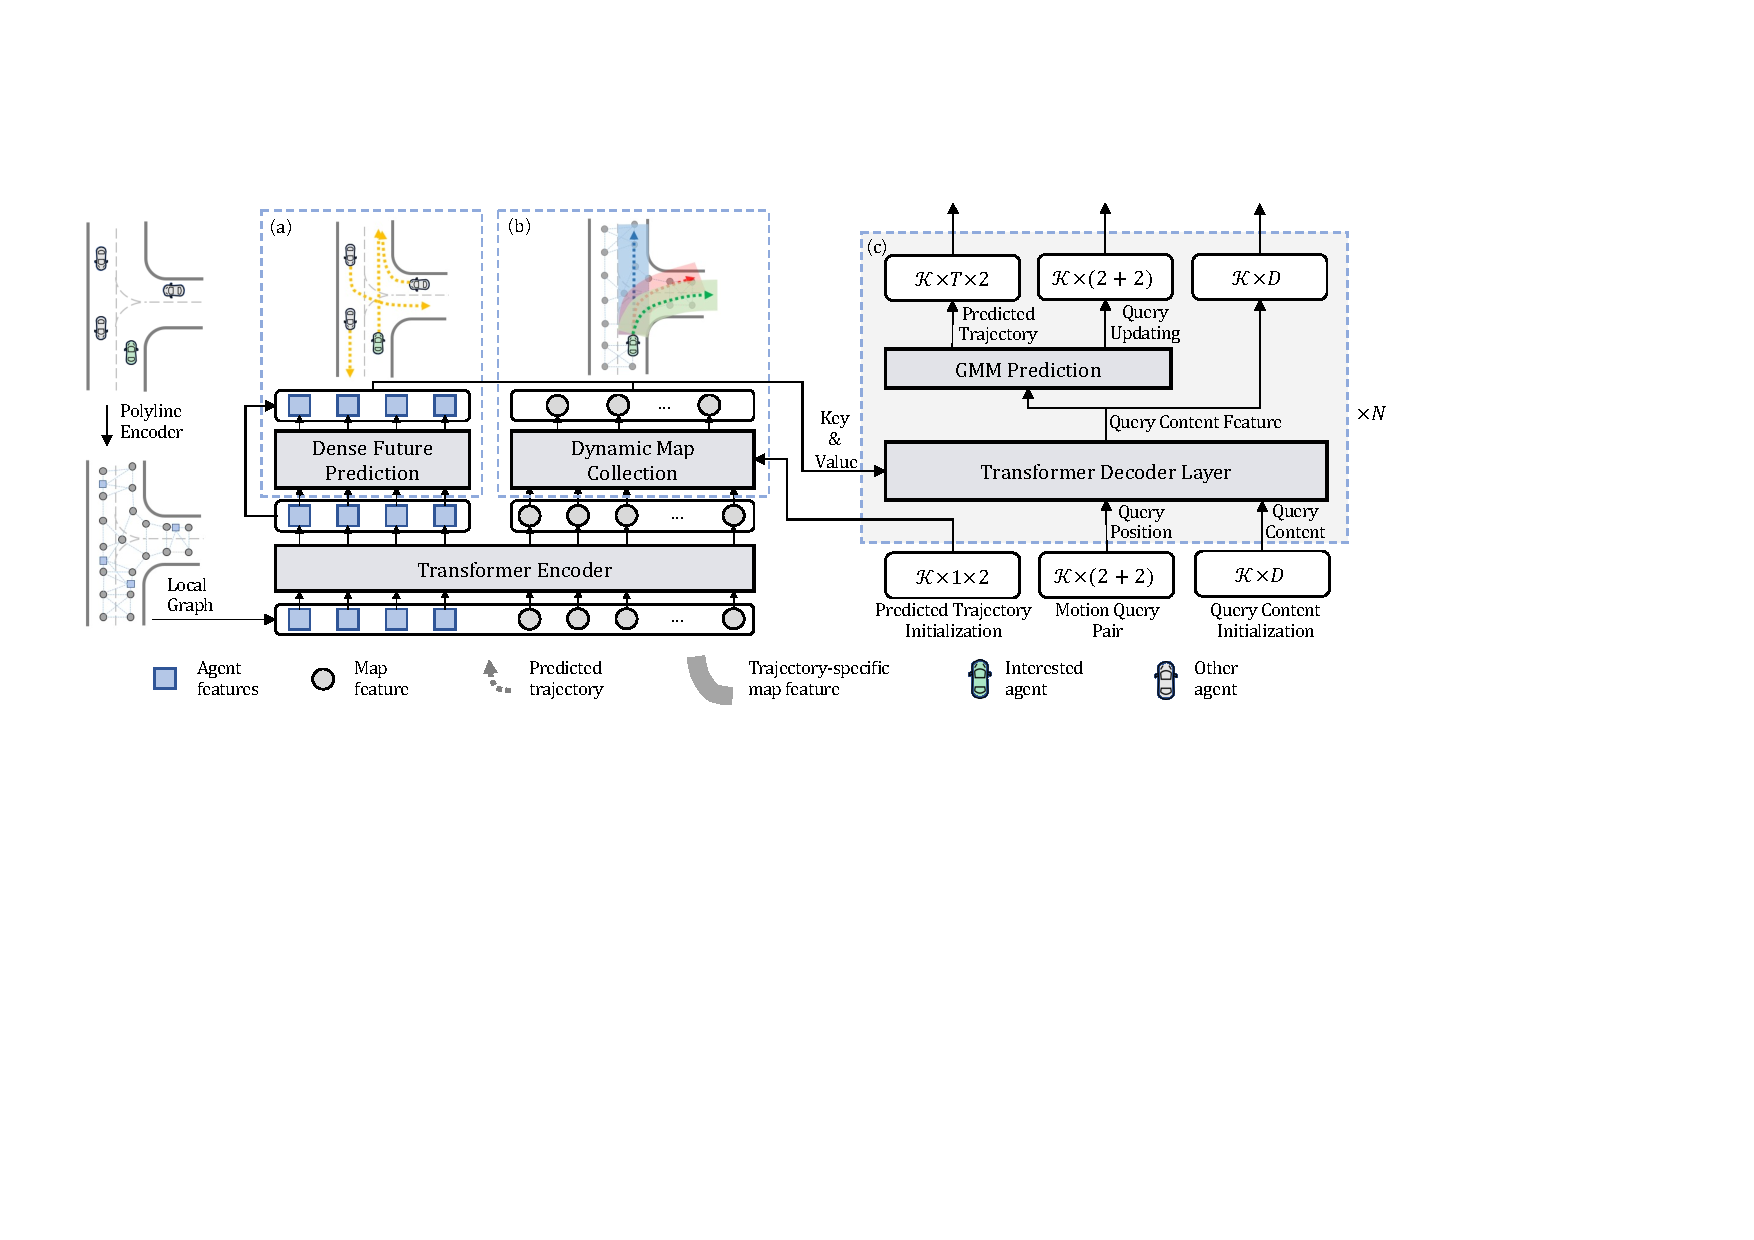
\includegraphics[width=0.96\linewidth]{figures/framework_mtr.pdf}\\
%		\vspace{-0.1in}
		\caption{
		MTR框架的整体架构。（a）密集未来预测（Dense Future Prediction）模块，为每个智能体预测单一轨迹（如上图中黄色虚线所示）。
		（b）动态地图收集（Dynamic Map Collection）模块，沿每条预测轨迹收集地图元素（如上图中沿轨迹的阴影区域所示），为运动解码器网络提供轨迹特化特征。
		（c）运动解码器网络，其中$\mathcal{K}$为运动查询对数量，$T$为未来帧数，$D$为隐藏特征维度，$N$为Transformer解码器层数。
		预测轨迹、运动查询对和查询内容特征均为上一解码器层输出，并作为下一解码器层的输入。对于第一解码器层，运动查询对的两个组成部分均初始化为预定义的意图点，预测轨迹由意图点替代以进行初始地图收集，查询内容特征初始化为零。
	}
		\label{fig:framework}
%		\vspace{-3mm}
	\end{figure*}
	
	%############################### Method Section####################################
%	\vspace{-1mm}
	\section{运动Transformer（Motion TRansformer, MTR）}
    \vspace{-3mm}
	本文提出运动Transformer（MTR），采用新型Transformer编码器-解码器结构，通过迭代运动精炼预测多模态未来运动。
		整体结构如图~\ref{fig:framework}所示。
	第~\ref{sec:encoder}节介绍用于场景上下文建模的编码器网络。
	第~\ref{sec:decoder}节介绍具有运动查询对新概念的运动解码器网络，用于预测多模态轨迹。
	最后，第~\ref{sec:training_loss}节介绍框架的优化过程。
	
%	\vspace{-2mm}
	\subsection{用于场景上下文建模的Transformer编码器}\label{sec:encoder}
	\vspace{-2mm}
	智能体的未来行为高度依赖于智能体之间的交互和道路地图。
	为编码这类场景上下文，现有方法通过构建全局交互图~\cite{gao2020vectornet,gu2021densetnt}或将地图特征汇总为智能体维度特征~\cite{ngiam2021scene,varadarajan2021multipath++}等方式进行了多种探索。
	本文认为局部性结构对编码场景上下文至关重要，尤其是对道路地图。
	%
	因此，提出一种具有局部自注意力（Local Self-Attention）的Transformer编码器网络，以更好地保持这种结构信息。
	
	\myparagraph{输入表示（Input Representation）.}
	遵循向量化表示~\cite{gao2020vectornet}，将输入轨迹和道路地图均组织为折线（Polyline）。
	对于目标智能体的运动预测，采用以智能体为中心（Agent-Centric）的策略~\cite{zhao2020tnt,gu2021densetnt,varadarajan2021multipath++}，将所有输入归一化到以该智能体为中心的坐标系。然后，
	采用简单的折线编码器将每条折线编码为Transformer编码器的输入令牌特征。
	%
	具体而言，将$N_a$个智能体的历史状态记为$A_{\text{in}}\in \mathbb{R}^{N_a\times t \times C_a}$，其中$t$为历史帧数，$C_a$为状态信息维度（\emph{例如}位置、朝向角和速度），对帧数不足$t$的轨迹在缺失帧位置补零。
	道路地图记为$M_{\text{in}}\in \mathbb{R}^{N_m\times n \times C_m}$，其中$N_m$为地图折线数量，$n$为每条折线的点数，$C_m$为每个点的属性数量（\emph{例如}位置和道路类型）。
	两者均通过类似PointNet~\cite{qi2017pointnet}的折线编码器编码如下：
	\begin{align}\label{eq:polyline}
		A_{\text{p}} = \phi\left(\text{MLP}(A_{\text{in}})\right),~~~~ M_{\text{p}} = \phi\left(\text{MLP}(M_{\text{in}})\right), 
	\end{align}
	其中$\text{MLP}(\cdot)$为多层感知机网络，$\phi$为最大池化操作，
	将每条折线特征汇总为智能体特征$A_{\text{p}}\in \mathbb{R}^{N_a\times D}$和地图特征$M_{\text{p}} \in \mathbb{R}^{N_m\times D}$，特征维度为$D$。
	
	\myparagraph{基于局部Transformer编码器的场景上下文编码（Scene Context Encoding with Local Transformer Encoder）.}
	场景上下文的局部结构对运动预测很重要。
	例如，两条平行车道的关系对建模变道行为很重要，但在全局连接图上使用注意力会平等考虑所有车道的关系。
	相比之下，将这种先验知识引入上下文编码器，采用局部注意力，更好地保持了局部性结构，且内存效率更高。
	具体而言，第$j$个Transformer编码器层的注意力模块可表示为：
	\begin{align}
	\small
		G^j = \text{MultiHeadAttn}\left(\text{query=}G^{j-1}+\text{PE}_{G^{j-1}}, ~\text{key=}\kappa(G^{j-1})+\text{PE}_{\kappa(G^{j-1})}, ~\text{value=}\kappa(G^{j-1})\right),
	\end{align}
	其中$\text{MultiHeadAttn}(\cdot, \cdot, \cdot)$为多头注意力（Multi-Head Attention）层~\cite{vaswani2017attention}，
	$G^0=[A_{\text{p}}, M_{\text{p}}]\in\mathbb{R}^{(N_a+N_m)\times D}$为智能体和地图特征的拼接，
	$\kappa(\cdot)$表示k近邻（$k$-Nearest Neighbor）算法，为每个查询折线找到k条最近的折线。
	$\text{PE}$表示输入令牌的正弦位置编码（Sinusoidal Position Encoding），其中对每个智能体使用其最新位置，对每条地图折线使用其折线中心。
	得益于这种局部自注意力，本文框架可以编码更大范围的场景上下文。
	
	编码器网络最终生成智能体特征$A_{\text{past}}\in \mathbb{R}^{N_a\times D}$和地图特征$M\in \mathbb{R}^{N_m\times D}$，
	作为后续解码器网络的场景上下文输入。
	
    \myparagraph{面向未来交互的密集未来预测（Dense Future Prediction for Future Interactions）.}
	与其他智能体的交互会严重影响目标智能体的行为，先前工作提出通过基于中心-主机的网络~\cite{zhu2019starnet}、动态关系推理~\cite{li2020evolvegraph}、社交时空网络~\cite{xu2021tra2tra}等方式建模多智能体交互。然而，大多数现有工作通常专注于学习历史轨迹上的交互，而忽略了未来轨迹的交互。
	因此，考虑到编码特征$A$已学习了所有智能体的丰富上下文信息，
	提出在$A$上采用简单的回归头来密集预测所有智能体的未来轨迹和速度：
	\begin{align}\label{eq:aux_reg}
		S_{1:T}=\text{MLP}(A_{\text{past}}),
	\end{align}
	其中$S_{i} \in \mathbb{R}^{N_a\times 4}$包含每个智能体在时间步$i$的未来位置和速度，$T$为待预测的未来帧数。
	预测轨迹$S_{1:T}$通过采用与式~\eqref{eq:polyline}相同的折线编码器将智能体的未来状态编码为特征$A_{\text{future}}\in \mathbb{R}^{N_a\times D}$，
	然后通过特征拼接和三层MLP对上述特征$A$进行增强：
	$A=\text{MLP}([A_{\text{past}}, A_{\text{future}}])$。
	该辅助任务为解码器网络提供额外的未来上下文信息，有助于模型为目标智能体预测更符合场景的未来轨迹。
	表~\ref{tab:ab_exp}的实验表明这一简洁轻量的辅助任务能有效提升多模态运动预测的性能。
	
%	\vspace{-2mm}
	\subsection{基于运动查询对的Transformer解码器}\label{sec:decoder}
	\vspace{-2mm}
	在给定场景上下文特征后，采用基于Transformer的运动解码器网络进行多模态运动预测，其中提出\emph{运动查询对（Motion Query Pair）}将运动预测建模为全局意图定位与局部运动精炼的联合优化。
	每个运动查询对包含两类查询：\emph{即}静态意图查询（Static Intention Query）和动态搜索查询（Dynamic Searching Query），分别用于全局意图定位和局部运动精炼。
    %
	如图~\ref{fig:decoder}所示，运动解码器网络包含多个堆叠的Transformer解码器层，用于通过运动查询对迭代精炼预测轨迹。
	下面说明其详细结构。
	
	
	\myparagraph{全局意图定位（Global Intention Localization）}旨在高效准确地定位智能体的潜在运动意图。
	提出\emph{静态意图查询（Static Intention Query）}，通过为不同运动模式使用不同的意图查询来缩小未来轨迹的不确定性。
	具体而言，
		\begin{wrapfigure}{r}{0.50\textwidth}
		\centering
		\vspace{-3mm}
		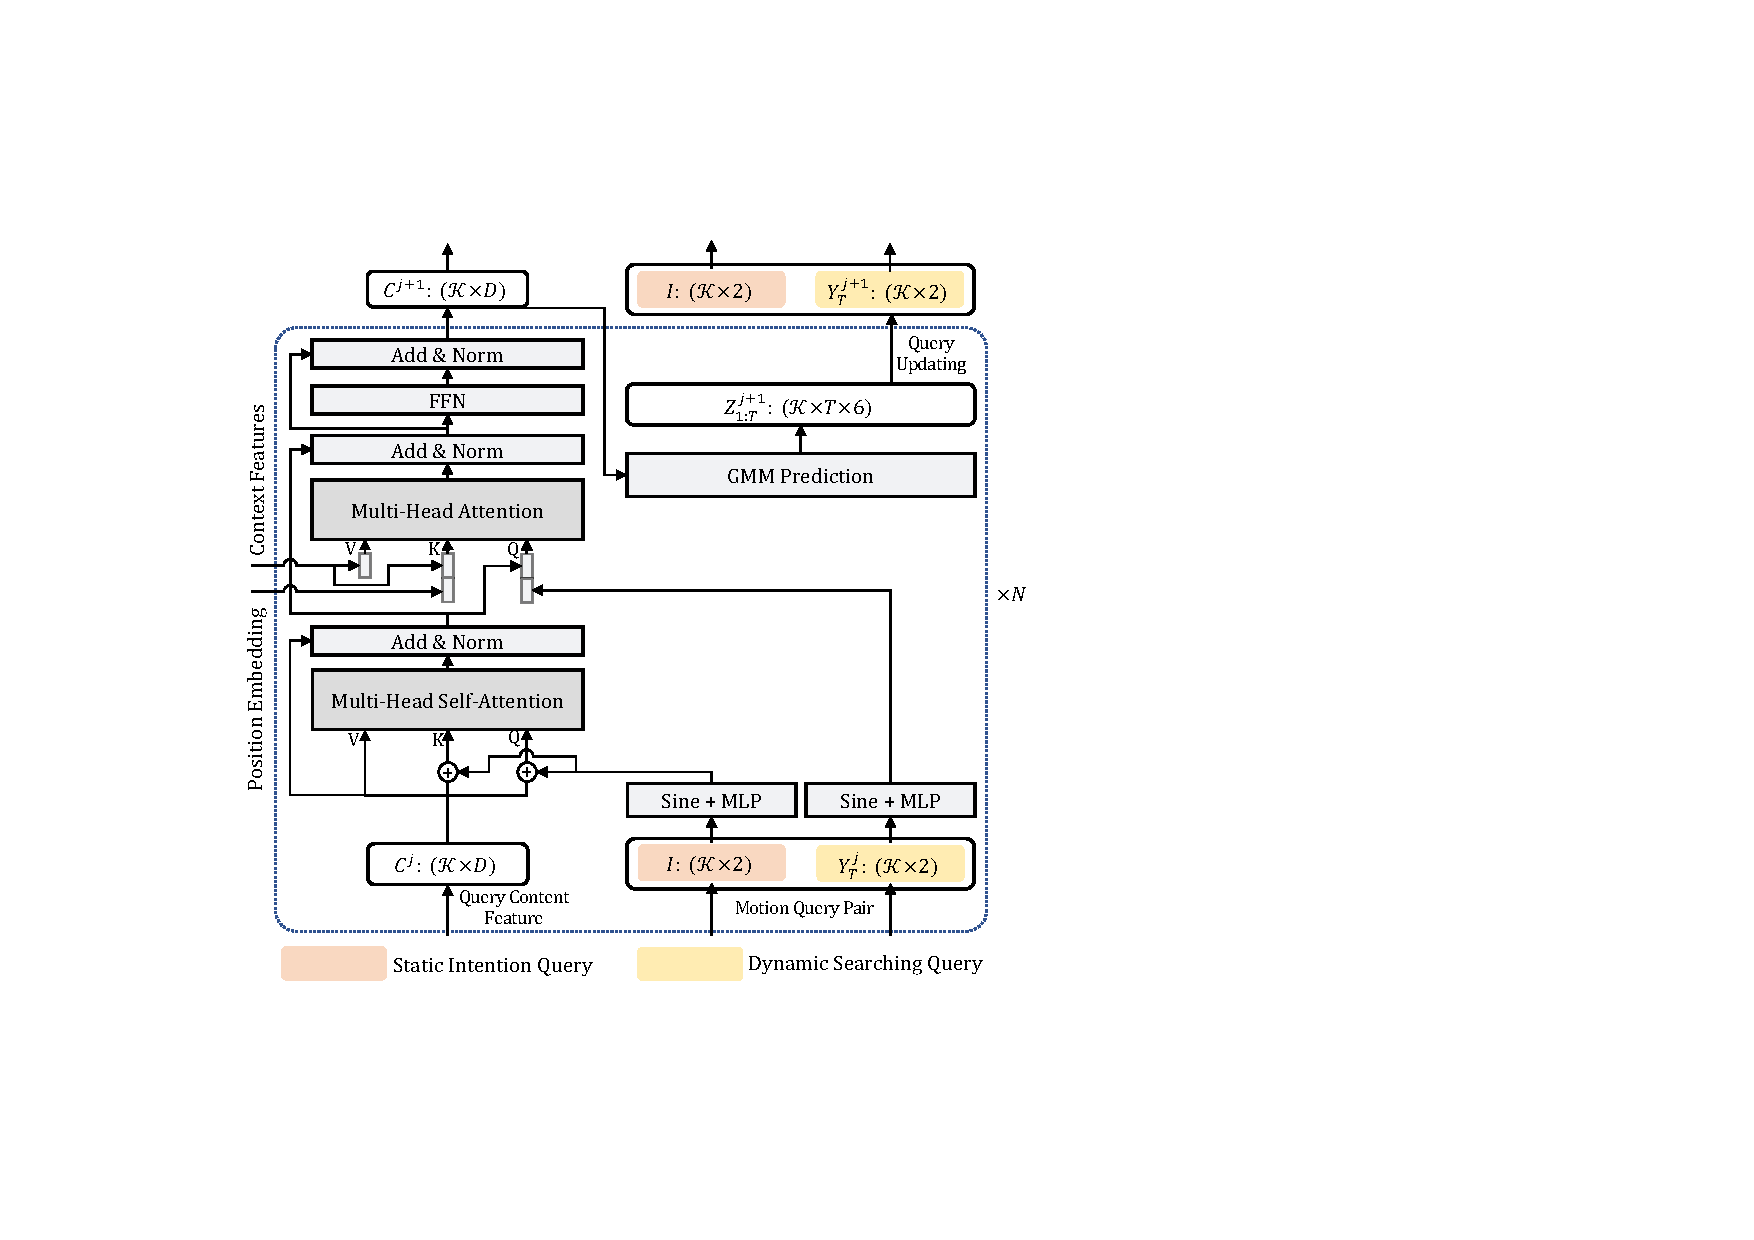
\includegraphics[width=0.53\textwidth]{figures/motion_decoder.pdf}
		\vspace{-6mm}
		\caption{\small 带有运动查询对的运动解码器网络结构。}
		\label{fig:decoder}
		\vspace{0mm}
	\end{wrapfigure}
	通过k均值聚类（k-Means Clustering）算法在真实值（Ground-Truth, GT）轨迹的端点上得到$\mathcal{K}$个代表性意图点$I\in \mathbb{R}^{\mathcal{K}\times 2}$，
	每个意图点表示同时考虑运动方向和速度的隐式运动模式。
	将每个静态意图查询建模为意图点的可学习位置嵌入：
	\begin{align}
		Q_I = \text{MLP}\left(\text{PE}(I)\right),
	\end{align}
	其中\text{PE}($\cdot$)为正弦位置编码，$Q_I \in \mathbb{R}^{\mathcal{K}\times D}$。
	%
	每个意图查询负责预测特定运动模式的轨迹，由于每种运动模式拥有自己的可学习嵌入，这稳定了训练过程并有助于预测多模态轨迹。
	得益于其可学习和自适应的特性，仅需少量查询（\emph{例如}本设置中为64个查询）即可实现高效的意图定位，无需使用密集排列的目标候选点~\cite{zhao2020tnt,gu2021densetnt}来覆盖智能体的目的地。
	
	\myparagraph{局部运动精炼（Local Movement Refinement）}旨在通过迭代收集细粒度轨迹特征来精炼轨迹，以补充全局意图定位。
	提出\emph{动态搜索查询（Dynamic Searching Query）}，为每个运动模式自适应地探查轨迹特征。
	每个动态搜索查询也是空间点的位置嵌入，初始化为对应的意图点，但在每个解码器层中会依据预测轨迹动态更新。
	%
	具体而言，给定第$j$个解码器层的预测未来轨迹$Y^j_{1:T}=\{Y^j_i \in \mathbb{R}^{\mathcal{K} \times 2}\mid i=1, \cdots, T\}$，第$(j+1)$个解码器层的动态搜索查询更新如下：
	\begin{align}
		Q_S^{j+1} = \text{MLP}\left(\text{PE}(Y^j_T)\right).
	\end{align}
	如图~\ref{fig:map_pool}所示，针对每个运动查询对，提出\emph{动态地图收集（Dynamic Map Collection）}模块，通过从轨迹对齐的局部区域查询地图特征来提取细粒度轨迹特征，
	具体通过收集$L$条中心点最接近预测轨迹的折线来实现。
	由于智能体行为高度依赖道路地图，这种局部运动精炼策略能够持续关注最新的局部上下文信息以进行迭代运动精炼。

	\myparagraph{基于运动查询对的注意力模块（Attention Module with Motion Query Pair）.}
	在每个解码器层中，静态意图查询用于在不同运动意图之间传播信息，而动态搜索查询用于从场景上下文特征中聚合轨迹特化特征。
	%
	具体而言，将静态意图查询用作自注意力（Self-Attention）模块的位置嵌入：
	\begin{align}\label{eq:decoder_sa}
		C_{\text{sa}}^j = \text{MultiHeadAttn}(\text{query=} C^{j-1} + Q_I, ~\text{key=}C^{j-1} + Q_I, ~\text{value=}C^{j-1}),
	\end{align}
	其中$C^{j-1} \in \mathbb{R}^{\mathcal{K}\times D}$为来自第$(j-1)$个解码器层的查询内容特征，$C^0$初始化为零，$C_{\text{sa}}^j\in \mathbb{R}^{\mathcal{K}\times D}$为更新后的查询内容。
	%
	接下来，利用动态搜索查询作为交叉注意力（Cross-Attention）的查询位置嵌入，从编码器输出中探查轨迹特化特征。
	受\cite{meng2021conditional,liu2022dabdetr}启发，将查询和键的内容特征与位置嵌入拼接，以解耦它们对注意力权重的贡献。
	分别采用两个交叉注意力模块来聚合智能体特征$A$和地图特征$M$的特征：
	\begin{align}\label{eq:decoder_ca}
		C^j_{A} &= \text{MultiHeadAttn}(\text{query=} [C_{\text{sa}}^j, Q_S^j], ~\text{key=} [A, \text{PE}_A], ~\text{value=}A),\nonumber\\
		C^j_{M} &= \text{MultiHeadAttn}(\text{query=} [C_{\text{sa}}^j, Q_S^j], ~\text{key=} [\alpha(M), \text{PE}_{\alpha(M)}], ~\text{value=} \alpha(M)),\\
		C^j &= \text{MLP}([C^j_{A}, C^j_{M}])\nonumber
	\end{align}
	其中$[\cdot, \cdot]$表示特征拼接，$\alpha(M)$为前述的动态地图收集模块，用于收集$L$条轨迹对齐的地图特征以进行运动精炼。
	为简洁起见，在式~\eqref{eq:decoder_sa}和\eqref{eq:decoder_ca}中省略了Transformer层~\cite{vaswani2017attention}中的残差连接（Residual Connection）和前馈网络（Feed-Forward Network）。
	
	最终，$C^j\in \mathbb{R}^{\mathcal{K}\times D}$为第$j$层中每个运动查询对的更新后查询内容特征。
		
	\begin{figure*}[t]
		\centering
		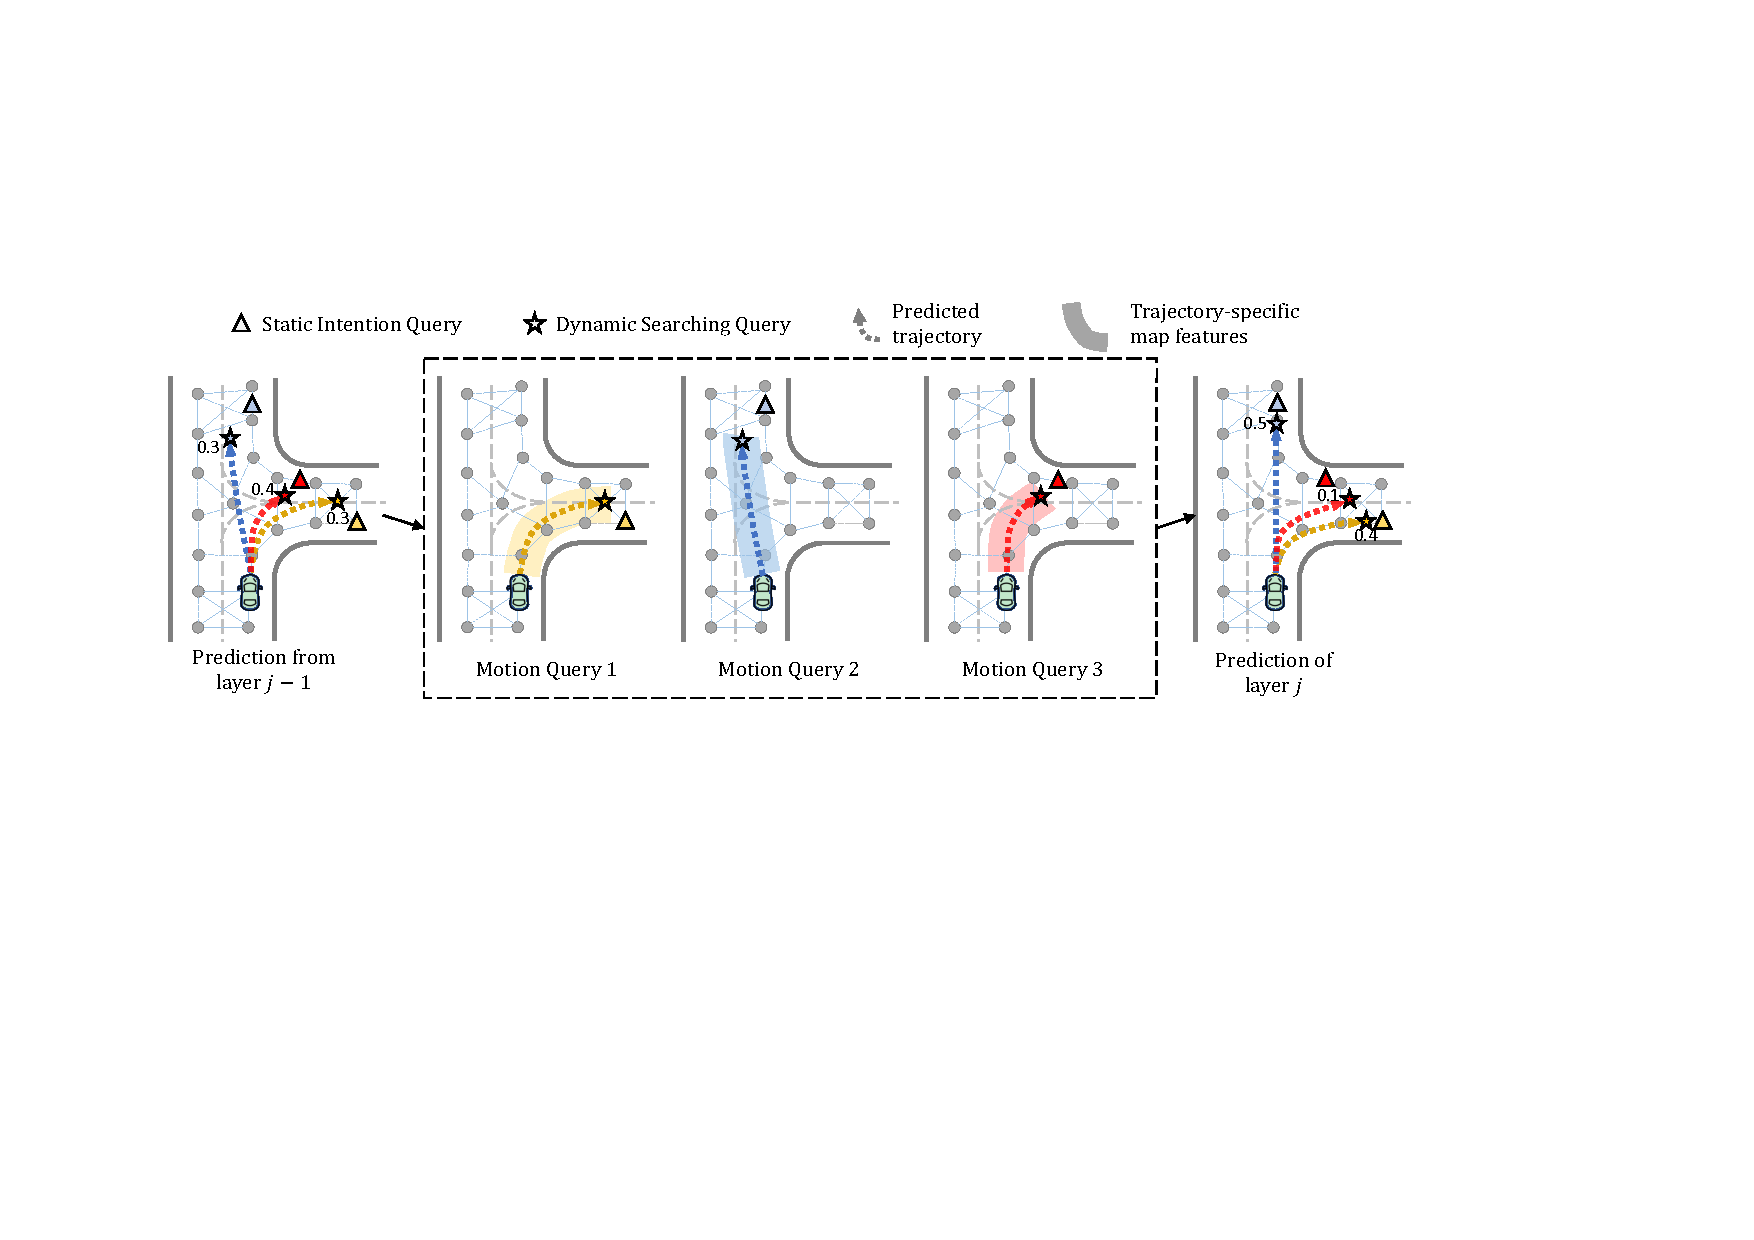
\includegraphics[width=0.99\linewidth]{figures/dynamic_map_collection.pdf}\\
%		\vspace{-0.1in}
		\caption{
			动态地图收集模块的示意图，用于迭代运动精炼。
		}
		\label{fig:map_pool}
%		\vspace{-3mm}
	\end{figure*}
	
	
	\myparagraph{基于高斯混合模型的多模态运动预测（Multimodal Motion Prediction with Gaussian Mixture Model）.}
	对每个解码器层，在$C^j$上附加预测头以生成未来轨迹。
	由于智能体行为高度多模态，遵循\cite{chai2019multipath,varadarajan2021multipath++}的做法，在每个时间步使用高斯混合模型（Gaussian Mixture Model, GMM）表示预测轨迹的分布。
	具体而言，对每个未来时间步$i\in \{1, \cdots, T\}$，预测每个高斯分量的概率$p$和参数（$\mu_x, \mu_y, \sigma_x, \sigma_y, \rho$）：
	\begin{align}\label{eq:gau_reg}
		Z^j_{1:T} = \text{MLP}(C^j),
	\end{align}
	其中$Z^j_{i}\in \mathbb{R}^{\mathcal{K}\times6}$包含$\mathcal{K}$个高斯分量$\mathcal{N}_{1:\mathcal{K}}(\mu_x, \sigma_x; \mu_y, \sigma_y; \rho)$及其概率分布$p_{1:\mathcal{K}}$。 
	智能体在时间步$i$的预测位置分布可表示为：
	\begin{align}\label{eq:gau_prob}
		P^j_i(o) = \sum_{k=1}^{\mathcal{K}}p_k\cdot\mathcal{N}_k(o_x-\mu_x, \sigma_x;o_y - \mu_y, \sigma_y;\rho).
	\end{align}
	其中$P^j_i(o)$为智能体在空间位置$o\in \mathbb{R}^{2}$的出现概率。
	预测轨迹$Y^j_{1:T}$可通过直接提取高斯分量的预测中心生成。
    
%    \vspace{-2mm}
	\subsection{训练损失}\label{sec:training_loss}\vspace{-2mm}
	本文模型采用端到端方式训练，包含两个训练损失。
	第一个辅助损失是$L1$回归损失，用于优化式~\eqref{eq:aux_reg}的输出。
	第二个高斯回归损失采用负对数似然（Negative Log-Likelihood）损失，根据式~\eqref{eq:gau_prob}最大化真实轨迹的似然。
	%
	受\cite{chai2019multipath,varadarajan2021multipath++}启发，
    采用硬分配（Hard-Assignment）策略，选择一个最近的运动查询对作为正高斯分量进行优化，选择方式是通过计算每个意图点与GT轨迹端点之间的距离来实现。
	高斯回归损失在每个解码器层中均被采用，最终损失为辅助回归损失与所有高斯回归损失之和，各损失权重相等。
	更多损失细节请参考附录。

	\section{实验}\vspace{-2mm}
	\subsection{实验设置}\label{sec:exp_setup}
	\vspace{-2mm}
	\myparagraph{数据集与评估指标（Dataset and Metrics）.}
	本文方法在大规模Waymo开放运动数据集（WOMD）~\cite{ettinger2021large}上进行评估，该数据集从真实交通场景中挖掘有趣的交互实例，是当前最多样化的交互式运动数据集。
	WOMD包含两个任务，分别使用不同的评估指标：
	（1）\emph{边缘运动预测挑战（Marginal Motion Prediction Challenge）}独立评估每个智能体的预测运动（每个场景最多8个智能体）。
	（2）\emph{联合运动预测挑战（Joint Motion Prediction Challenge）}需要预测两个交互智能体的联合未来位置以进行评估。
	两者均提供1秒历史数据，旨在预测未来8秒内智能体的6条边缘或联合轨迹。
    %
	各任务共有$487k$个训练场景，约$44k$个验证场景和$44k$个测试场景。
	利用官方评估工具计算评估指标，
	其中mAP和漏检率（Miss Rate）是官方排行榜~\cite{womd_leaderboard,womd_leaderboard_interact}中最关键的指标。
	
	\myparagraph{实现细节（Implementation Details）.}
	上下文编码方面，堆叠6个Transformer编码器层。
	道路地图表示为多条折线，每条折线最多包含20个点（在WOMD中约$10m$）。
	选择目标智能体周围最近的$N_m=768$条地图折线。
	编码器局部自注意力的邻居数设为16。
	编码器隐藏特征维度设为$D=256$。
	%
	解码器模块方面，堆叠6个解码器层。
	$L$设为128，从上下文编码器收集最近的地图折线用于运动精炼。
	默认使用64个运动查询对，其意图点
	通过在训练集上执行k均值聚类算法生成。
	为生成用于评估的6条未来轨迹，使用非极大值抑制（Non-Maximum Suppression, NMS），通过计算端点距离从64条预测轨迹中选出前6条，距离阈值设为$2.5m$。
    更多细节请参考附录。
	
	\myparagraph{训练细节（Training Details）.}
	采用AdamW优化器以端到端方式训练，学习率为0.0001，批大小为80个场景。
	使用8块GPU（NVIDIA RTX 8000）训练30个周期，从第20周期开始每2个周期将学习率衰减0.5倍。
	权重衰减设为0.01，不使用任何数据增强。
	
	\myparagraph{面向端到端运动预测的MTR-e2e（MTR-e2e for End-to-End Motion Prediction）.}
	还提出MTR的端到端变体MTR-e2e，
	仅采用6个运动查询对以去除NMS后处理。
	在训练过程中，MTR-e2e不像MTR那样使用静态意图点进行目标分配，
	而是通过计算其6条预测轨迹与GT轨迹之间的距离来选择正混合分量，因为6个意图点过于稀疏，难以充分覆盖所有潜在的未来运动。
	
	\begin{table*}
		\centering\small
		\setlength\tabcolsep{9pt}
		\caption{在Waymo开放运动数据集验证集和测试集上的边缘运动预测性能对比。
        $\dagger$：斜体结果仅供参考，因其通过模型集成技术获得。
		受WOMD提交次数限制，仅将默认设置MTR提交至官方测试服务器进行测试集评估。}
		\vspace{1mm}
		\resizebox{0.99\textwidth}{!}{
			\begin{tabular}{c|l|c||ccccc}
				\hline
				\rowcolor{mygray} & Method & Reference & minADE~$\downarrow$ & minFDE~$\downarrow$ & Miss Rate~$\downarrow$ & {\bf mAP}~$\uparrow$ \\
				\hline
				 \multirow{6}{*}{Test} & MotionCNN~\cite{konev2021motioncnn} & CVPRw 2021 & 0.7400 & 1.4936 & 0.2091 & 0.2136  \\
				& ReCoAt~\cite{huangrecoat} & CVPRw 2021 & 0.7703 & 1.6668 & 0.2437 & 0.2711	 \\
				& DenseTNT~\cite{gu2021densetnt} & ICCV 2021 & 1.0387 & 1.5514 & 0.1573 & 0.3281  \\
				& SceneTransformer~\cite{ngiam2021scene} & ICLR 2022 & 0.6117 & {\bf 1.2116} & 0.1564 & 0.2788 \\ 
				& MTR (Ours) & - & {\bf0.6050} & 1.2207 & {\bf0.1351} &{\bf0.4129}	 \\
				\cline{2-7} 
				& $^\dagger$MultiPath++~\cite{varadarajan2021multipath++} & ICRA 2022 & \emph{0.5557} & \emph{1.1577}
				& \emph{0.1340} & \emph{0.4092}  \\
				& $^\dagger$MTR-Advanced-ens (Ours) & - & {\it 0.5640} & {\it 1.1344} & {\it 0.1160} & {\it 0.4492}\\
				\hline 
				\multirow{3}{*}{Val} & MTR (Ours) & - & 0.6046 & 1.2251 & 0.1366 & {\bf 0.4164} \\
				& MTR-e2e (Ours) & - &  {\bf 0.5160} & {\bf 1.0404} & {\bf 0.1234} & 0.3245	\\
				\cline{2-7}
				& $^\dagger$MTR-ens (Ours) & - & {\it 0.5686} & {\it 1.1534} & {\it 0.1240} & {\it 0.4323}	\\ 
				& $^\dagger$MTR-Advanced-ens (Ours) & - &  {\it 0.5597} & {\it 1.1299} & {\it 0.1167} & {\it 0.4551} \\
				\hline
		\end{tabular}
		}
		\vspace{-3mm}
		\label{tab:wod_test}
	\end{table*}

    \begin{table*}
		\centering\small
		\setlength\tabcolsep{7pt}
		\caption{在Waymo开放运动数据集交互式验证集和测试集上的联合运动预测性能对比。}
		\vspace{1mm}
		\resizebox{0.99\textwidth}{!}{
			\begin{tabular}{c|l|c||ccccc}
				\hline
				\rowcolor{mygray} & Method & Reference & minADE~$\downarrow$ & minFDE~$\downarrow$ & Miss Rate~$\downarrow$ & { \bf mAP}~$\uparrow$ \\
				\hline
				\multirow{6}{*}{Test}& Waymo LSTM baseline~\cite{ettinger2021large} & ICCV 2021 & 1.9056 & 5.0278 & 0.7750 & 0.0524  \\
				& HeatIRm4~\cite{mo2021multi} & CVPRw 2021 & 1.4197 & 3.2595 & 0.7224 & 0.0844 \\
				& AIR$^2$~\cite{wu2021air} & CVPRw 2021 & 1.3165 & 2.7138 & 0.6230 & 0.0963 \\ 
				& SceneTransformer~\cite{ngiam2021scene} & ICLR 2022 & 0.9774 & 2.1892 & 0.4942 & 0.1192 \\ 
				& M2I~\cite{sun2022m2i} & CVPR 2022 & 1.3506 & 2.8325 & 0.5538 & 0.1239\\ 
				& MTR (Ours) & - & {\bf 0.9181} & {\bf 2.0633} & {\bf 0.4411}	 & {\bf 0.2037}	\\
				\hline 
				\multirow{1}{*}{Val}& MTR (Ours) & - & 0.9132 & 2.0536	& 0.4372 & 0.1992\\
				\hline
		\end{tabular}
		}
		\vspace{-3mm}
		\label{tab:wod_interactive}
	\end{table*}

%	\vspace{-2mm}
	\subsection{主要结果}\vspace{-2mm}
	\myparagraph{边缘运动预测性能对比（Performance Comparison for Marginal Motion Prediction）.}
	表~\ref{tab:wod_test}展示了边缘运动预测的主要结果，
	    MTR显著超越了此前无集成方法~\cite{gu2021densetnt,ngiam2021scene}，mAP提升+$8.48\%$，漏检率从$15.64\%$降至$13.51\%$。
	值得注意的是，MTR的单模型结果在mAP上也优于最新工作MultiPath++~\cite{varadarajan2021multipath++}，后者采用了新颖的模型集成策略来提升性能。
	
	表~\ref{tab:wod_test}还展示了MTR变体的对比。MTR-e2e通过去除NMS后处理获得了更好的minADE和minFDE，而MTR由于学习了每个运动查询对的显式含义，能产生更置信的意图预测，从而获得更好的mAP。
	%
	还提出简单的模型集成策略，合并MTR和MTR-e2e的预测并使用NMS去除冗余预测（记为MTR-ens），该策略融合了两者的优势，实现了更优的mAP。
	将此集成策略应用于框架的7个变体（\emph{例如}更多解码器层、不同查询数量、更大隐藏维度）后，高级集成结果（记为MTR-Advanced-ens）在测试集排行榜上取得了最佳性能。
	 
	
	\myparagraph{联合运动预测性能对比（Performance Comparison for Joint Motion Prediction）.} 为评估联合运动预测性能，遵循\cite{casas2020implicit,ettinger2021large,sun2022m2i}的方法，将两个交互智能体的边缘预测结合为联合预测，从这两个智能体的$36$种组合中取前6个联合预测。每个组合的置信度为边缘概率的乘积。
	表~\ref{tab:wod_interactive}显示本文方法在所有指标上大幅超越现有最优方法~\cite{ngiam2021scene,sun2022m2i}。特别是MTR将mAP从$12.39\%$提升至$20.37\%$，漏检率从$49.42\%$降至$44.11\%$。
	显著的性能提升证明了MTR在预测场景一致的未来轨迹方面的有效性。
    此外，在图~\ref{fig:demo}中展示了一些定性结果，显示在复杂交互场景中的预测效果。
	
	截至2022年5月19日，MTR在WOMD两个挑战的运动预测排行榜上均排名第一~\cite{womd_leaderboard,womd_leaderboard_interact}。
	基于更多集成变体的MTR方法（\textit{即}MTR-Advacned-ens）还获得了Waymo开放数据集挑战赛2022运动预测挑战赛冠军~\cite{womd_leaderboard2022,shi2022mtr}。
	这些显著提升证明了MTR框架的有效性。 
	
	\begin{table*}
		\centering\small
		\setlength\tabcolsep{2pt}
		\caption{MTR框架中各组件的效果。所有模型共享相同的编码器网络。``latent learnable embedding''表示使用6个潜在可学习嵌入作为解码器网络的查询，``iterative refinement''表示使用6个堆叠解码器进行运动精炼。}
		\resizebox{0.999\textwidth}{!}{
			\begin{tabular}{cccc|cccc}
				\hline
				\rowcolor{mygray}\tabincell{c}{Global Intention\\ Localization}& \tabincell{c}{Iterative \\Refinement} & \tabincell{c}{Local Movement \\Refinement} & \tabincell{c}{Dense Future \\Prediction} & minADE~$\downarrow$ & minFDE~$\downarrow$& Miss Rate~$\downarrow$ & {\bf mAP}~$\uparrow$ \\
				\hline 
				Latent learnable embedding & $\times$ & $\times$ & $\times$ & 0.6829 & 1.4841 & 0.2128 & 0.2633	\\
				Static intention query & $\times$ &  $\times$ & $\times$ & 0.7036 & 1.4651 & 0.1845 & 0.3059 \\
				Static intention query & $\checkmark$ & $\times$ & $\times$ &  0.6919 & 1.4217 & 0.1776 & 0.3171\\
				Static intention query &$\checkmark$ & $\checkmark$ & $\times$ & 0.6833 & 1.4059 & 0.1756 & 0.3234	\\
				Static intention query & $\checkmark$  & $\times$ & $\checkmark$& 0.6735 & 1.3847 & 0.1706 &0.3284	\\
				Static intention query & $\checkmark$ & $\checkmark$ & $\checkmark$ & {\bf 0.6697} & {\bf1.3712} & {\bf0.1668} &{\bf0.3437}\\
				\hline
			\end{tabular}
		}
		\label{tab:ab_exp}
%		\vspace{-5mm}
	\end{table*}
	
	
%	\vspace{-2mm}
	\subsection{消融实验}\label{sec:exp_ab}\vspace{-3mm}
	研究MTR中各组件的有效性。
	为高效进行消融实验，按照默认顺序从WOMD训练集中均匀采样$20\%$的数据（约$97k$个场景），实验发现其与完整训练集的分布相似。
	所有模型均在WOMD验证集上使用边缘运动预测指标进行评估。
	
	\myparagraph{运动解码器网络的影响（Effects of the Motion Decoder Network）.}
	研究解码器网络中各组件的有效性，包括全局意图定位、迭代精炼和局部运动精炼。
	表~\ref{tab:ab_exp}显示所有组件对最终性能（以官方排名指标mAP衡量）均有显著贡献。
	特别是，提出的带意图点的静态意图查询相比潜在可学习嵌入取得了更优的mAP（\emph{即}+$4.26\%$），这得益于其模式特化的查询策略；迭代精炼和局部运动精炼策略通过聚合更细粒度的轨迹特征进行运动精炼，将mAP从$30.59\%$持续提升至$32.34\%$。
	
	
	\myparagraph{密集未来预测的影响（Effects of Dense Future Prediction）.}
	表~\ref{tab:ab_exp}表明密集未来预测模块显著提升了预测轨迹的质量（\emph{例如}+$1.78\%$ mAP），验证了智能体轨迹的未来交互对运动预测的重要性，且本文策略能够学习此类交互以预测更可靠的轨迹。
	

	
	\setcounter{figure}{2}
	\begin{figure}
		\centering
		\subfigure{
			\begin{minipage}{0.55\linewidth}
				\centering
				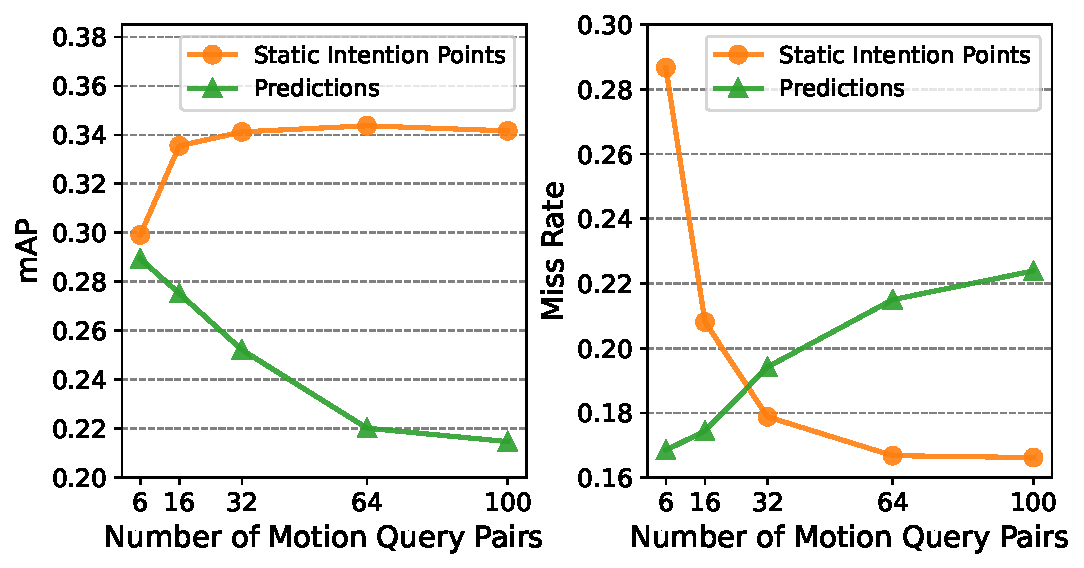
\includegraphics[width=0.99\linewidth]{figures/exp_target_assignment.pdf}
				\vspace{-0.75cm}
				\captionof{figure}{MTR框架在不同运动查询对数量下的表现，两条不同颜色的线展示了训练过程中选择正混合分量的两种策略。}
				\label{fig:ab_num_queries}
%				\vspace{-4mm}
			\end{minipage}
		}%
		\subfigure{
			\begin{minipage}{0.42\linewidth}
				\centering
				\setlength\tabcolsep{2pt}
				\makeatletter\def\@captype{table}\makeatother
				\captionof{table}{Transformer编码器中局部自注意力的效果。``\#polyline''是用于上下文编码的输入地图折线数量，折线数量多表示目标智能体周围有更大的地图上下文。``OOM''表示内存耗尽。}
				\vspace{1mm}
				\resizebox{0.999\textwidth}{!}{
					\begin{tabular}{cc|cccc}
						\hline
						\rowcolor{mygray}Attention & \#Polyline &  minADE~$\downarrow$ & minFDE~$\downarrow$& MR~$\downarrow$ & {\bf mAP}~$\uparrow$ \\
						\hline
						Global & 256 & 0.683 & 1.4031 & 0.1717	 & 0.3295	\\
						Global & 512 & 0.6783 & 1.4018 & 0.1716 & 0.3280	\\
						Global & 768 & OOM & OOM & OOM & OOM \\
						\hline 
						Local & 256 & 0.6724 & 1.3835 & 0.1683 & 0.3372\\
						Local & 512 & 0.6707 & 1.3749 & 0.1670 & 0.3392\\
						Local & 768 & {\bf0.6697} & {\bf1.3712} & 0.1668 & 0.3437 \\
						Local & 1024 & 0.6757 & 1.3782 & {\bf0.1663} & {\bf0.3452} \\
						\hline
					\end{tabular}
				}
				\label{tab:ab_local_attn}
%				\vspace{-4mm}
			\end{minipage}
		}%
		\vspace{-3mm}
		\centering
	\end{figure}
	
			
	\setcounter{figure}{4}
	\begin{figure*}[t]
		\centering
		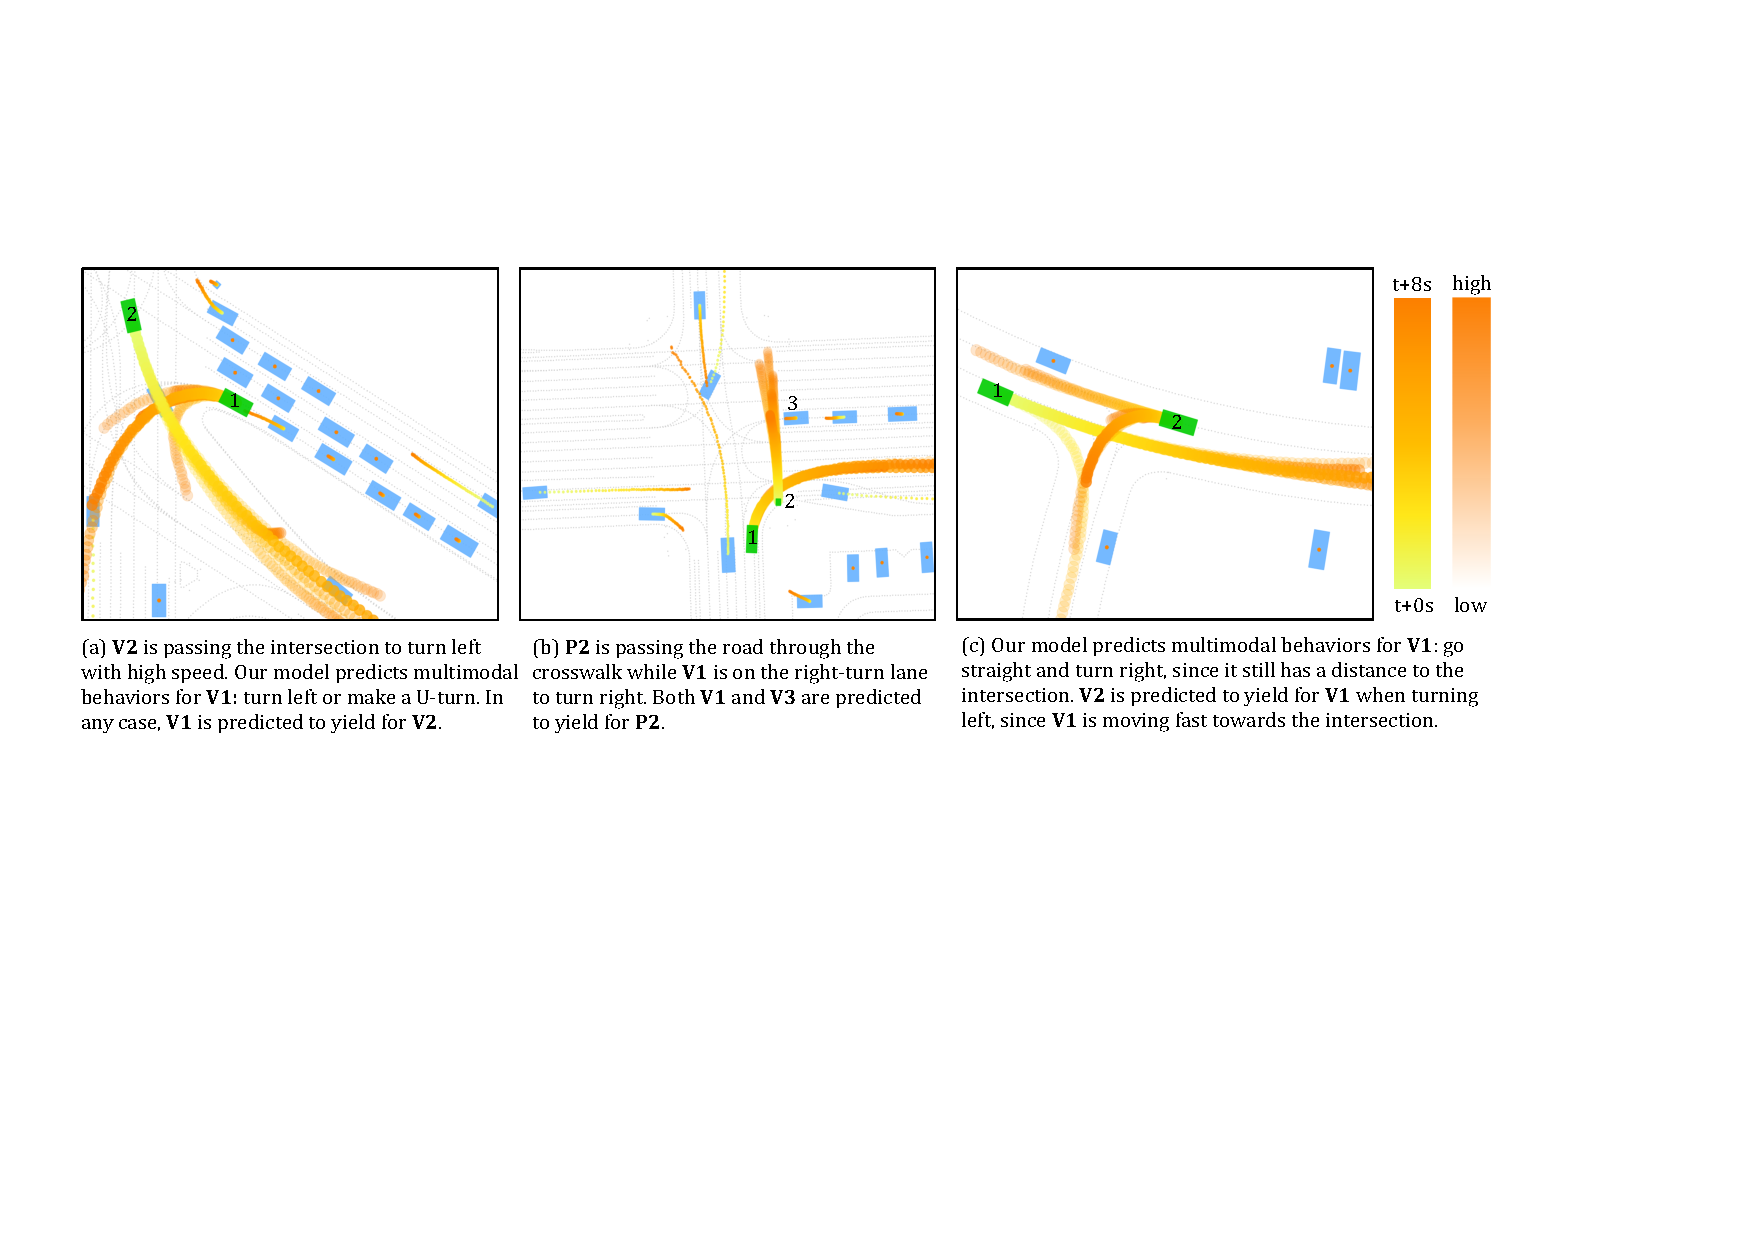
\includegraphics[width=0.99\linewidth]{figures/mtr_demo.pdf}\\
% 		\vspace{-0.1in}
%		\vspace{-3mm}
		\caption{
			MTR框架在WOMD上的定性结果。
			每个场景中有两个目标智能体（绿色矩形），模型为每个目标智能体预测6条多模态未来轨迹。对其他智能体（蓝色矩形），密集未来预测模块预测单条轨迹。
			使用渐变色可视化不同未来时间步的轨迹路点，轨迹置信度通过不同透明度展示。缩写：车辆（{\bf V}）、行人（{\bf P}）。
		}
		\label{fig:demo}
%		\vspace{-5mm}
	\end{figure*}
	
	
	\myparagraph{上下文编码中局部注意力的影响（Effects of Local Attention for Context Encoding）.}
	表~\ref{tab:ab_local_attn}显示，在输入相同数量地图折线的情况下，Transformer编码器中的局部自注意力比全局注意力取得了更优性能（\emph{即}256条折线时mAP提升+$0.77\%$，512条折线时提升+$1.12\%$），验证了输入局部结构对运动预测的重要性，通过局部注意力引入此类先验知识有助于提升性能。
	更重要的是，局部注意力内存效率更高，当地图折线数量从256增加到1,024时性能持续增长，而全局注意力因其二次复杂度会耗尽内存。
	
	\noindent
	{\bf 不同训练策略下运动查询对数量的影响（Effects of the Number of Motion Query Pairs with Different Training Strategies）.}
	如前所述，在训练过程中，MTR和MTR-e2e采用两种不同的正混合分量分配策略，MTR依赖静态意图点（记为$\alpha$），而MTR-e2e使用预测轨迹（记为$\beta$）。
	%
	图~\ref{fig:ab_num_queries}研究了这两种策略下运动查询对数量的影响，得到以下观察结果：
	%
	（1）当增加运动查询对数量时，
	策略$\alpha$相比策略$\beta$取得了更好的mAP和漏检率。因为每个意图查询点负责特定的运动模式，可以确保更稳定的训练过程。相比之下，策略$\beta$依赖于不稳定的预测，正分量可能在所有分量间随机切换，因此大量运动查询对难以用策略$\beta$优化。
	（2）每个意图查询点的显式含义也解释了策略$\alpha$始终优于策略$\beta$的原因，因为它能以更置信的分数预测轨迹，从而提升mAP指标。
	%
	（3）另一方面，当减少运动查询对数量时，策略$\alpha$的漏检率大幅上升，因为有限数量的意图查询点无法充分覆盖智能体所有潜在运动。相反，策略$\beta$在少量运动查询对下表现良好，因为其查询不负责特定区域，可以全局适应任意区域。
	
	\vspace{-2mm}
	\section{结论}\label{sec:conclusion}\vspace{-4mm}
	本文提出MTR——一个用于多模态运动预测的新颖框架。
	运动查询对被定义为将运动预测建模为全局意图定位与局部运动精炼的联合优化。
	全局意图定位采用少量可学习的静态意图查询高效捕获智能体的运动意图，局部运动精炼则通过持续探查细粒度轨迹特征进行迭代运动精炼。
	在大规模WOMD数据集的边缘和联合运动预测挑战上的实验表明，本文方法达到了当前最优性能。
    
    \myparagraph{局限性（Limitations）.}
   本文框架采用以智能体为中心的策略预测单个目标智能体的多模态未来轨迹，导致同一场景中多个目标智能体的上下文编码存在冗余。
   因此，如何开发能够同时为多个智能体预测多模态运动的框架是未来工作的重要方向。此外，基于规则的后处理可能导致minADE和minFDE指标上的次优预测，如何设计更好的策略从完整的多模态预测（例如64个预测）中生成所需数量的未来轨迹（例如6条），也值得探索以构建更鲁棒的框架。

{\small
	\bibliographystyle{plain}
	\bibliography{egbib}
}


\clearpage 
\appendix


{\LARGE\bf 附录}
%\vspace{-3mm}
\section{实现细节}\label{sec:implement_details}
%\vspace{-3mm}
\myparagraph{更多架构细节（More Architecture Details）.}
训练单个模型预测所有三个类别（\emph{即}车辆、行人、骑行者）的未来运动，每个类别拥有各自的运动查询对。

输入历史状态$A_{\text{in}}$包含三类信息：智能体历史运动状态（\emph{即}位置、物体尺寸、朝向角和速度）、每个智能体的独热类别掩码以及每个历史时间步的独热时间嵌入。$A_{\text{in}}$的折线编码器包含三层MLP，特征维度为256。
%
输入地图特征$M_{\text{in}}$包含三类信息：每个折线点的位置、每个点的折线方向以及每条折线的类型。
$M_{\text{in}}$的折线编码器包含五层MLP，特征维度为64，由于地图折线数量远大于智能体数量，因此采用较小的特征维度。
两个折线编码器最终分别通过另一个线性层投影到256特征维度。


对于密集未来预测模块，采用三层MLP，中间特征维度为512，用于预测所有智能体的未来位置和速度。
对于每个解码器层中的预测头，采用三层MLP，中间特征维度为512，不同解码器层之间的模型权重不共享。

\myparagraph{高斯回归损失的细节（Details of Gaussian Regression Loss）.}
给定特定未来时间步的预测高斯混合模型，采用负对数似然损失最大化该时间步智能体真实位置$(\hat{Y}_x, \hat{Y}_y)$的似然，具体损失公式如下：
\begin{align}
    L_G&=-\log\mathcal{N}_h(\hat{Y}_x - \mu_x, \sigma_x; \hat{Y}_y - \mu_y, \sigma_y; \rho) - \text{log}(p_h)\\
    &=\log\sigma_x + \log\sigma_y + 0.5\log(1-\rho^2)+\frac{1}{2(1-\rho^2)}\left(\left(\frac{d_x}{\sigma_x}\right)^2+ \left(\frac{d_y}{\sigma_y}\right)^2 - 2\rho\frac{d_xd_y}{\sigma_x\sigma_y} \right)- \text{log}(p_h),\nonumber
\end{align}
其中$d_x=\hat{Y}_x-\mu_x$, $d_y=\hat{Y}_y-\mu_y$, $\mathcal{N}_h(\mu_x, \sigma_x; \mu_y, \sigma_y; \rho)$为选中的用于优化的正高斯分量。$p_h$是该选中正高斯分量的预测概率，在上式中采用交叉熵损失最大化选中正高斯分量的概率。

\myparagraph{最终训练损失（Final Training Losses）.}
根据上述高斯回归损失的定义，MTR框架的最终训练损失为各解码器层中所有高斯回归损失与辅助回归损失之和，各损失权重相等。


\begin{figure*}[h]
	\centering
	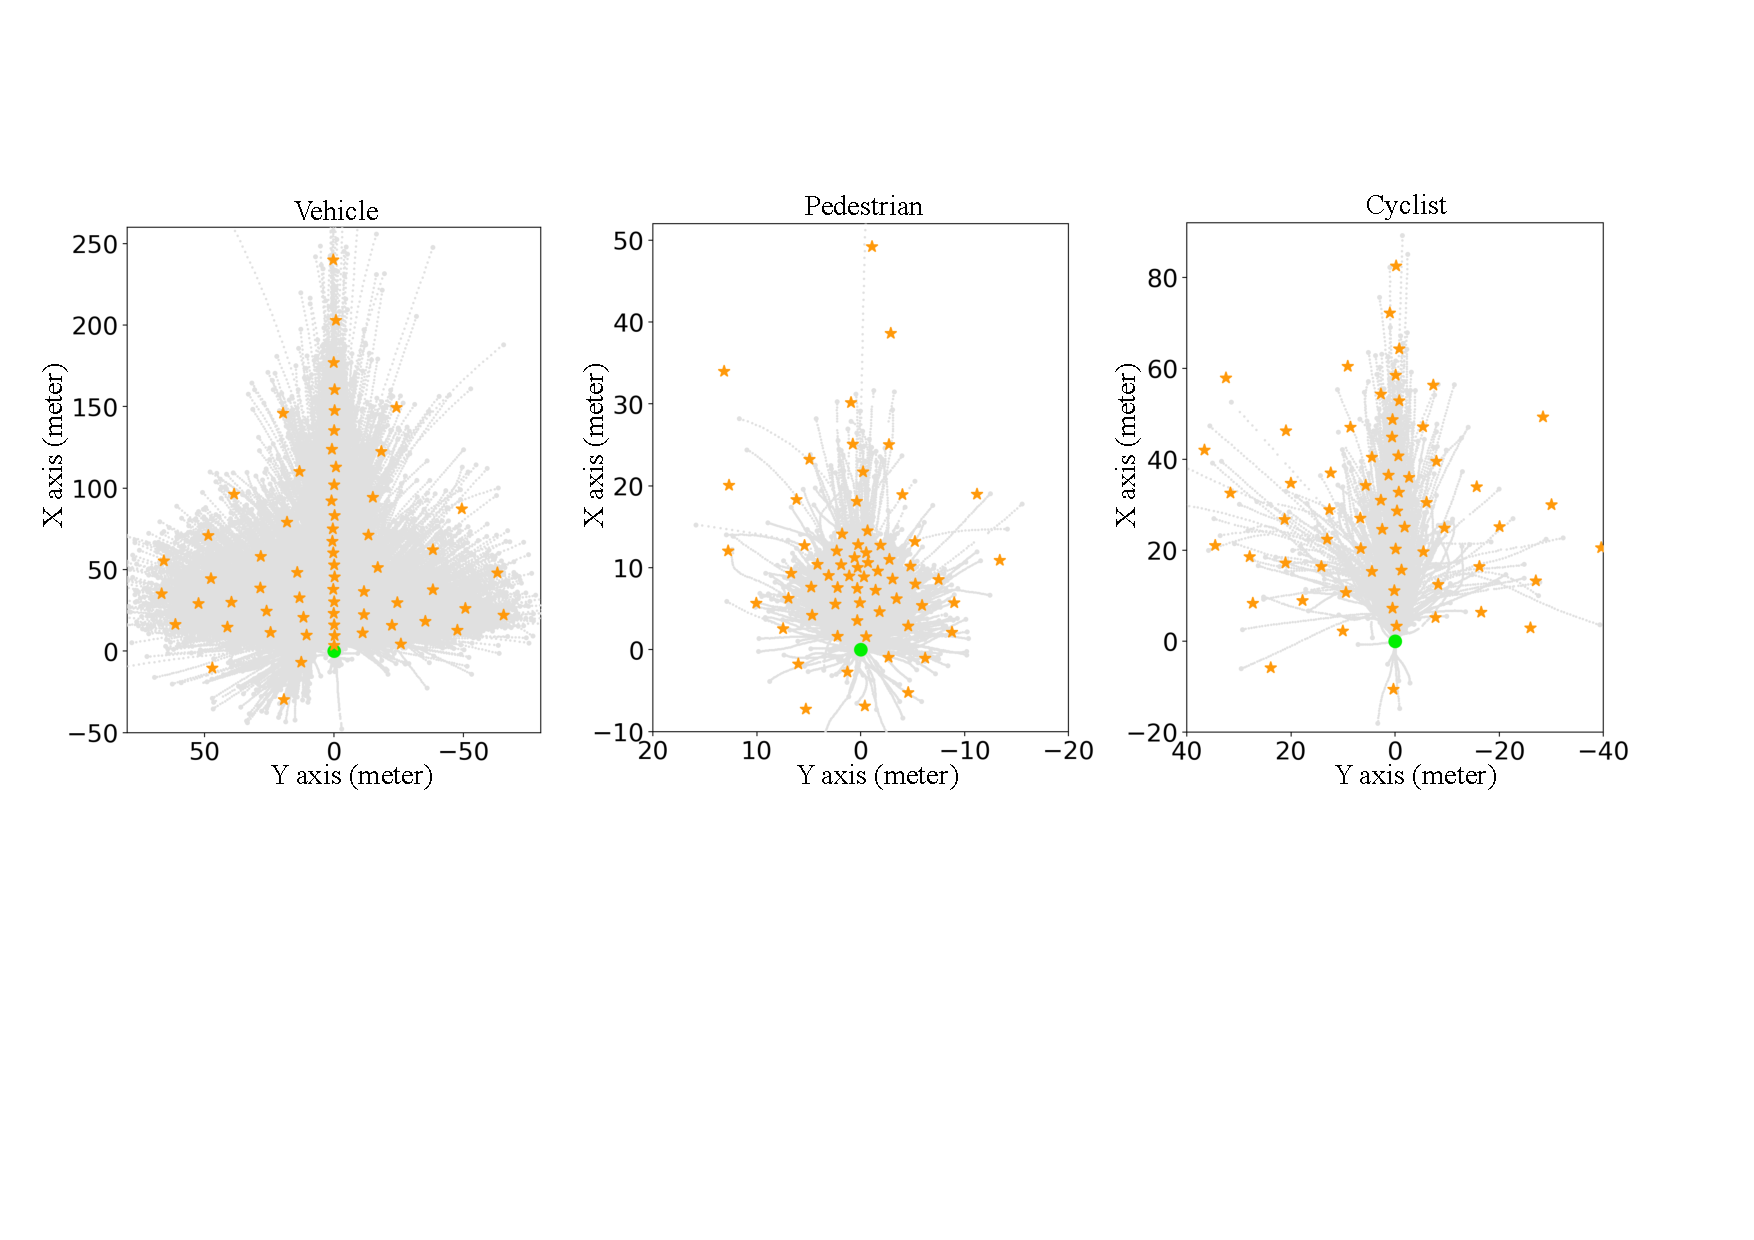
\includegraphics[width=0.99\linewidth]{figures/supp_intention_cluster.pdf}\\
% 		\vspace{-0.1in}
	\vspace{-2mm}
	\caption{各类别的静态意图点分布。绿色点为智能体当前位置，意图点以橙色星号表示。灰色虚线表示各类别真实轨迹的分布，为更好可视化，图中仅绘制了10\%的真实轨迹。}
	\label{fig:cluster}
	\vspace{-3mm}
\end{figure*}


\myparagraph{静态意图点的分布（Distribution of Static Intention Points）.}
如文中所述，采用k均值聚类算法为每个类别生成64个静态意图点。
如图~\ref{fig:cluster}所示，生成的意图点通过同时考虑未来运动的速度和方向，能够很好地覆盖大多数运动意图。
例如，车辆类别在前方向有一系列意图点，实际上建模了相同意图方向下不同速度的运动。 

    
\myparagraph{推理延迟（Inference Latency）.}
MTR在Waymo开放运动数据集的场景上平均推理延迟约为$59ms$（批大小为1）和$33ms$（批大小为6），模型为每个目标智能体（最多8个）预测6条多模态未来轨迹，并为所有其他智能体（最多128个）预测单条未来轨迹。该数据在NVIDIA RTX 8000上使用标准PyTorch代码测得。
    
\section{MTR框架的逐类别结果}\label{sec:per-class_performance}
如表~\ref{tab:wod_test_perclass}和\ref{tab:wod_test_perclass_interactive}所示，列出本文方法在Waymo开放运动数据集~\cite{ettinger2021large}边缘和联合运动预测挑战上的逐类别性能，供参考。

    \begin{table*}[h]
		\centering\small
		\setlength\tabcolsep{9pt}
		\caption{在Waymo开放运动数据集验证集和测试集上的边缘运动预测逐类别性能。$\dagger$：斜体结果仅供参考，因通过模型集成技术获得。}
		\vspace{1mm}
% 		\resizebox{0.99\textwidth}{!}{
			\begin{tabular}{c|l|c||ccccc}
				\hline
				\rowcolor{mygray} & Setting & Category & minADE~$\downarrow$ & minFDE~$\downarrow$ & Miss Rate~$\downarrow$ & { mAP}~$\uparrow$ \\
				\hline
				\multirow{4}{*}{Test}
				& \multirow{4}{*}{MTR} & Vehicle & 0.7642 & 1.5257	& 0.1514 & 0.4494	 \\
				& & Pedestrian & 0.3486 & 0.7270 & 0.0753 & 0.4331\\
				& & Cyclist & 0.7022 & 1.4093 & 0.1786 & 0.3561	 \\
				& & {\bf Avg} & 0.6050 & 1.2207 & 0.1351 & 0.4129	 \\
				\cline{1-7}
				\multirow{12}{*}{Val}
				& \multirow{4}{*}{MTR} & Vehicle & 0.7665 & 1.5359 & 0.1527	 & 0.4534	\\
				& & Pedestrian & 0.3456 & 0.7260 & 0.0741 & 0.4364	\\
				& & Cyclist & 0.7016 & 1.4134 & 0.1830 & 0.3594\\
				& & {\bf Avg} & 0.6046 & 1.2251 & 0.1366 & 0.4164\\
				\cline{2-7}
				& \multirow{4}{*}{MTR-e2e} & Vehicle & 	0.6087 & 1.2161 & 0.1160 & 0.3708 \\
				& & Pedestrian & 0.3046 &	0.6254	& 0.0696 & 0.3028	\\
				& & Cyclist & 0.6346 & 1.2796 & 0.1845 & 0.2998	 \\
				& & {\bf Avg} & 0.5160 & 1.0404 & 0.1234 & 0.3245\\
				\cline{2-7}
				\hline
		\end{tabular}
% 		}
		\vspace{-3mm}
		\label{tab:wod_test_perclass}
	\end{table*}
    
     \begin{table*}[h]
		\centering\small
		\setlength\tabcolsep{9pt}
		\caption{在Waymo开放运动数据集验证集和测试集上的联合运动预测逐类别性能。}
		\vspace{1mm}
			\begin{tabular}{c|l|c||ccccc}
				\hline
				\rowcolor{mygray} & Setting & Category & minADE~$\downarrow$ & minFDE~$\downarrow$ & Miss Rate~$\downarrow$ & { mAP}~$\uparrow$ \\
				\hline
				\multirow{4}{*}{Test}
				& \multirow{4}{*}{MTR} & Vehicle & 0.9793 & 2.2157 & 0.3833 & 0.2977\\
				& & Pedestrian & 0.7098 & 1.5835 & 0.3973 & 0.2033	 \\
				& & Cyclist & 1.0652 & 2.3908 & 0.5428 & 0.1102		 \\
				& & {\bf Avg} &{0.9181} & {2.0633} & {0.4411}	 & {0.2037}	 \\
				\cline{1-7}
				\multirow{4}{*}{Val}
				& \multirow{4}{*}{MTR} & Vehicle & 0.9675 & 2.1728 & 0.3722 & 0.3018		\\
				& & Pedestrian & 0.7097 & 1.5522 & 0.3984 & 0.1892		\\
				& & Cyclist & 1.0623 & 2.4357 & 0.5410 & 0.1065	 \\
				& & {\bf Avg} & 0.9132 & 2.0536	& 0.4372 & 0.1992\\
				\hline
		\end{tabular}
		\label{tab:wod_test_perclass_interactive}
% 		\vspace{-2mm}
	\end{table*}
    
    \begin{table*}[t]
		\centering\small
		\setlength\tabcolsep{9pt}
		\caption{在Waymo开放运动数据集验证集上的密集未来预测性能。密集未来预测模块为验证集中每个智能体预测单一未来轨迹（未来8秒）。ADE为平均位移误差，FDE为最终位移误差。FDE基于未来8秒的最后一个时间步评估，漏检率基于不同距离阈值下的FDE评估。}
		\vspace{1mm}
% 		\resizebox{0.99\textwidth}{!}{
			\begin{tabular}{c|cccc}
				\hline
				\rowcolor{mygray} Category & ADE~$\downarrow$ & FDE~$\downarrow$ & \tabincell{c}{Miss Rate\\ (thresh=$2m$)}~$\downarrow$ & \tabincell{c}{Miss Rate\\(thresh=$6m$)}~$\downarrow$ \\
				\hline
				Vehicle & 0.8755 & 3.4929 & 0.3343 & 0.1984\\ 
				Pedestrian & 0.4998 & 1.9685 & 0.3317 & 0.0601 \\ 
				Cyclist & 1.6565 & 6.3868 & 0.7697 & 0.3747 \\ 
				\textbf{Avg} & 1.0106 & 3.9494 & 0.4786 & 0.2111\\
				\hline
		\end{tabular}
% 		}
% 		\vspace{-3mm}
		\label{tab:wod_dense_future_prediction}
% 		\vspace{-2mm}
	\end{table*}

    	
	\begin{table*}[t]
		\centering\small
		\setlength\tabcolsep{9pt}
		\caption{与Argoverse2数据集测试集排行榜上前10名提交结果的性能对比。$K$为用于计算评估指标的预测轨迹数量。}
		\vspace{1mm}
% 		\resizebox{0.99\textwidth}{!}{
			\begin{tabular}{c|ccc}
				\hline
				\rowcolor{mygray}Method & Miss Rate ($K$=6)~$\downarrow$ & Miss Rate ($K$=1)~$\downarrow$ & brier-minFDE ($K$=6)~$\downarrow$ \\ 
				\hline
				MTR (Ours) & {\bf 0.15} & {\bf 0.58} & 1.98 \\
		    TENET~\cite{wang2022tenet} & 0.19 & 0.61 & {\bf 1.90}\\
			    OPPred & 0.19 & 0.60 & 1.92\\
			    Qml & 0.19 & 0.62 & 1.95\\
			    GANet & 0.17 & 0.60 & 1.97\\
                VI LaneIter & 0.19 & 0.61 & 2.00\\
                QCNet & 0.21 & 0.60 & 2.14\\
                THOMAS~\cite{gilles2021thomas} & 0.20 & 0.64 & 2.16\\
                HDGT~\cite{jia2022hdgt} & 0.21 & 0.66 & 2.24 \\ 
                GNA & 0.29 & 0.71 & 2.45\\
                vilab & 0.29 & 0.71 & 2.47\\
				\hline 
		\end{tabular}
% 		}
% 		\vspace{-3mm}
		\label{tab:argo2_test}
		\vspace{3mm}
	\end{table*}
	
    

    \section{密集未来预测评估}\label{sec:dense_future_prediction}
    如文中所述，提出密集未来预测模块以支持智能体之间的未来交互，其中所有邻近智能体的预测轨迹准确性对预测目标智能体更优的多模态轨迹至关重要。
    % 
    如表~\ref{tab:wod_dense_future_prediction}所示，简洁的密集未来预测模块能为所有智能体预测准确的未来轨迹，在8秒未来运动预测中$6.0m$距离阈值下的平均漏检率为$21.11\%$。
    值得注意的是，该漏检率是在为每个智能体仅预测一条未来轨迹的情况下实现的。
    虽然密集未来预测模块生成的轨迹仍不如解码器网络精确，
    但已通过实现智能体的未来交互为目标智能体的多模态运动预测带来益处。
    	

	\section{在Argoverse 2数据集上的性能对比}\label{sec:argo2}
	Argoverse 2运动预测数据集~\cite{wilson2021argoverse}是另一个大规模运动预测数据集，包含250,000个训练和验证场景。模型需要以每个场景的五秒历史数据作为输入，预测目标智能体未来六秒的轨迹，全程提供HDMap地图上下文信息。
	在此数据集上训练模型时，采用与Waymo数据集相同的超参数，只是模型以五秒历史轨迹为输入，需要预测六秒未来轨迹。
	
	将本文方法与Argoverse2数据集排行榜~\cite{argo2_leaderboard}上前10名提交结果进行对比，其中大多数提交是为Argoverse2运动预测竞赛2022定制的，竞争激烈。
	如表~\ref{tab:argo2_test}所示，MTR框架在漏检率相关指标上取得了显著的新的当前最优性能，展示了方法的强大泛化能力和鲁棒性。

	
	\begin{figure}[h]
    % \vspace{3mm}
		\centering
		\subfigure{
			\begin{minipage}{0.49\linewidth}
				\centering
				\makeatletter\def\@captype{table}\makeatother
				\captionof{table}{Transformer编码器中局部自注意力邻居数的影响。}
				\vspace{1mm}
				\resizebox{0.99\textwidth}{!}{
					\begin{tabular}{c|cccc}
						\hline
						\rowcolor{mygray}\#neighbors &  minADE~$\downarrow$ & minFDE~$\downarrow$& MR~$\downarrow$ & {\bf mAP}~$\uparrow$ \\
						4 & {\bf 0.6677} & 1.3724 & 0.1672 & 0.3405\\
						8 & 0.6681 & {\bf 1.3673} & 0.1670 & 0.3428\\ 
						16 & { 0.6697} & {1.3712} & {\bf 0.1668} & {\bf 0.3437} \\
						32 & 0.6701 & 1.3763 & 0.1678 & 0.3416	\\ 
						64 & 0.6727 & 1.3756 & 0.1687 & 0.3367\\ 
						\hline
					\end{tabular}
				}
				\label{tab:ab_neighbors}
				\vspace{-3mm}
			\end{minipage}
		}%
		\subfigure{
			\begin{minipage}{0.49\linewidth}
				\centering
				\makeatletter\def\@captype{table}\makeatother
				\captionof{table}{动态地图收集中地图折线数量的影响。}
				\vspace{1mm}
				\resizebox{0.999\textwidth}{!}{
					\begin{tabular}{c|cccc}
						\hline
						\rowcolor{mygray}\#Polyline &  minADE~$\downarrow$ & minFDE~$\downarrow$& MR~$\downarrow$ & {\bf mAP}~$\uparrow$ \\
						32 & 0.6735 & 1.3847 & 0.1701 & 0.3317\\ 
						64 & 0.6699 & {\bf 1.3650} & 0.1672 & 0.3386\\ 
						128 & {\bf 0.6697} & 1.3712 & 0.1668 & {\bf 0.3437} \\
				        256 & 0.6704 & 1.3729 & {\bf 0.1665} & 0.3396	\\
						\hline
					\end{tabular}
				}
				\label{tab:ab_map_polylines}
				\vspace{-3mm}
			\end{minipage}
		}%
% 		\vspace{-3mm}
		\centering
	\end{figure}
    
    \vspace{5mm}
    \section{更多消融实验}\label{sec:more_ab}
    
    \myparagraph{局部自注意力邻居数的影响（Effects of Number of Neighbors for Local Self-Attention）.}
    如表~\ref{tab:ab_neighbors}所示，在局部自注意力中使用4个邻居已在mAP上取得良好性能，且将邻居数从4增加到16时mAP持续增长。
    然而，将邻居数增加到64进行局部自注意力时，性能略有下降（\emph{即}从$34.37\%$降至$33.67\%$）。这表明少量邻居可以更好保持输入元素的局部结构，且更易于优化以获得更好性能，同时少量邻居在执行自注意力时计算和内存效率也远高于大量邻居。
    
    \myparagraph{动态地图收集中折线数量的影响（Effects of Number of Polylines for Dynamic Map Collection）.}
    表~\ref{tab:ab_map_polylines}显示，将收集的地图折线数量从32增加到128，可以通过以更大感受野检索轨迹特化的地图特征持续提升mAP。
    然而，收集256条地图折线进行轨迹精炼时性能略有下降（-$0.41\%$ mAP），表明收集更多地图折线可能引入更多噪声，无法提供精确的轨迹特化地图特征用于精炼。
    
    \begin{figure}[h]
        \vspace{-3mm}
		\centering
		\subfigure{
			\begin{minipage}{0.49\linewidth}
				\centering
				% \setlength\tabcolsep{2pt}
				\makeatletter\def\@captype{table}\makeatother
				\captionof{table}{解码器层数的影响。}
				\vspace{1mm}
				\resizebox{0.98\textwidth}{!}{
					\begin{tabular}{c|cccc}
						\hline
						\rowcolor{mygray}\#decoders &  minADE~$\downarrow$ & minFDE~$\downarrow$& MR~$\downarrow$ & {\bf mAP}~$\uparrow$ \\
						3 & 0.6717	& 1.3796 & 0.1686 & 0.3360 \\ 
						6 & { 0.6697} & {1.3712} & 0.1668 & {\bf 0.3437} \\
						9 & {\bf 0.6658} & {\bf 1.3621}	& {\bf 0.1661} & {\bf 0.3437}	\\
						\hline
					\end{tabular}
				}
				\label{tab:ab_decoder_number}
				% \vspace{-3mm}
			\end{minipage}
		}%
		\subfigure{
			\begin{minipage}{0.49\linewidth}
				\centering
				% \setlength\tabcolsep{2pt}
				\makeatletter\def\@captype{table}\makeatother
				\captionof{table}{静态意图点分布的影响。}
				\vspace{1mm}
				\resizebox{0.98\textwidth}{!}{
					\begin{tabular}{c|cccc}
						\hline
						\rowcolor{mygray} \#Distribution &  minADE~$\downarrow$ & minFDE~$\downarrow$& MR~$\downarrow$ & {\bf mAP}~$\uparrow$ \\ 
						uniform grids & 0.7214 & 1.5563 & 0.1970 & 0.3178\\  
						k-means & {\bf 0.6697} & {\bf 1.3712} & {\bf 0.1668} & {\bf 0.3437} \\
						
						\hline
					\end{tabular}
				}
				\label{tab:ab_anchor_initialize}
				% \vspace{-3mm}
			\end{minipage}
		}%
% 		\vspace{-1mm}
		\centering
	\end{figure}
    
    \myparagraph{解码器层数的影响（Effects of Number of Decoder Layers）.}
    表~\ref{tab:ab_decoder_number}显示，增加解码器层数可以持续提升性能，说明堆叠的Transformer解码器层能够通过不断聚合更精确的轨迹特化特征来迭代精炼预测轨迹。默认情况下，考虑到MTR框架性能与效率的权衡，采用6个解码器层。
    
    \myparagraph{静态意图点分布的影响（Effects of Distribution of Static Intention Points）.}
    如文中所述，采用k均值算法生成64个静态意图点作为运动查询对的基础。
    同时消融另一种简单的均匀采样策略，为每个类别生成相同数量的静态意图点，通过考虑各类别轨迹分布范围均匀采样$8\times8=64$个静态意图点（见图~\ref{fig:cluster}）。
    如表~\ref{tab:ab_anchor_initialize}所示，用均匀采样替代k均值算法生成静态意图点时性能显著下降。
    这验证了基于k均值的算法能产生更好的静态意图点分布，能够以少量静态意图点捕获更精确、更完整的未来运动意图。图~\ref{fig:cluster}也展示了默认静态意图点在捕获多模态运动意图方面的有效性。
    
    	
	
	\section{定性结果}\label{sec:more_figs}
    在图~\ref{fig:demo_supp}中提供更多MTR框架的定性结果。
    
    \begin{figure*}[h]
		\centering
		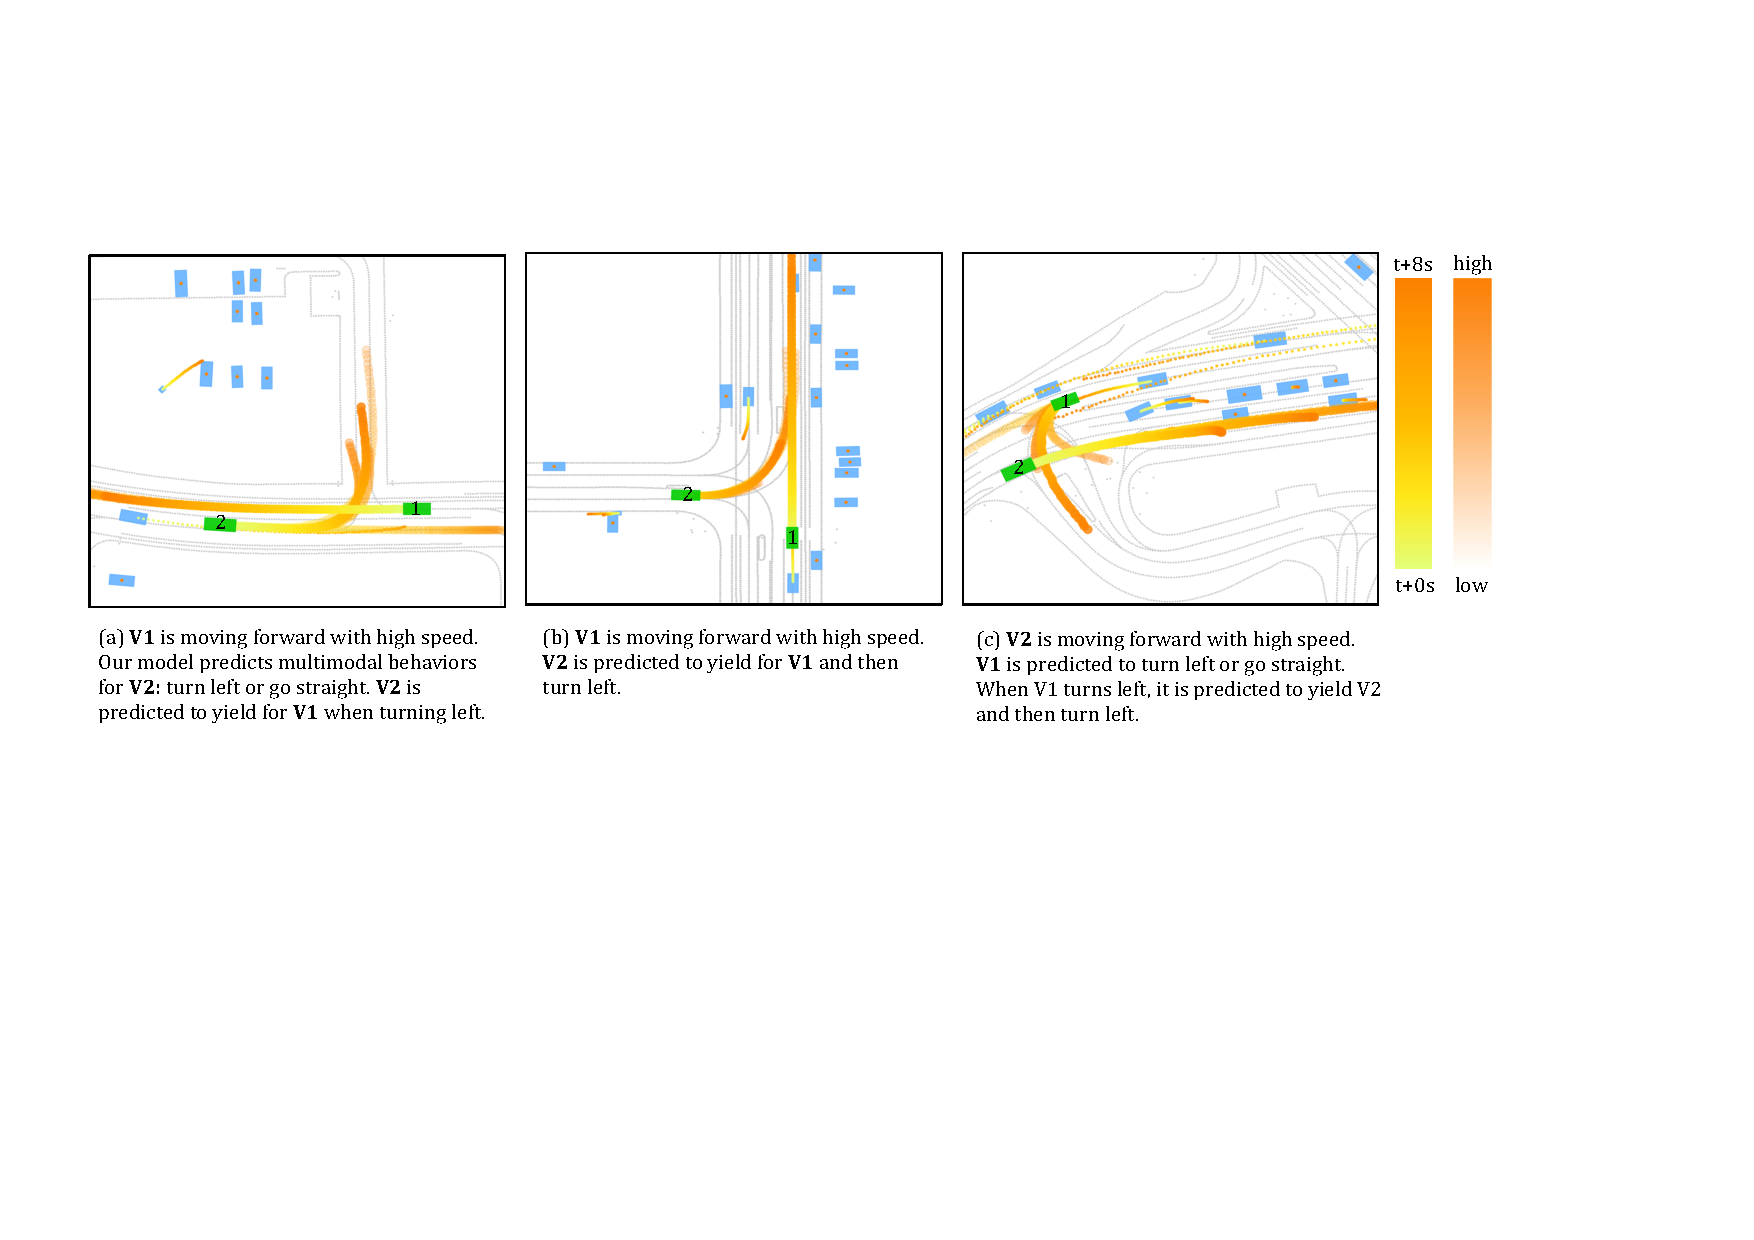
\includegraphics[width=0.99\linewidth]{figures/supp_demo_1.pdf}\\
		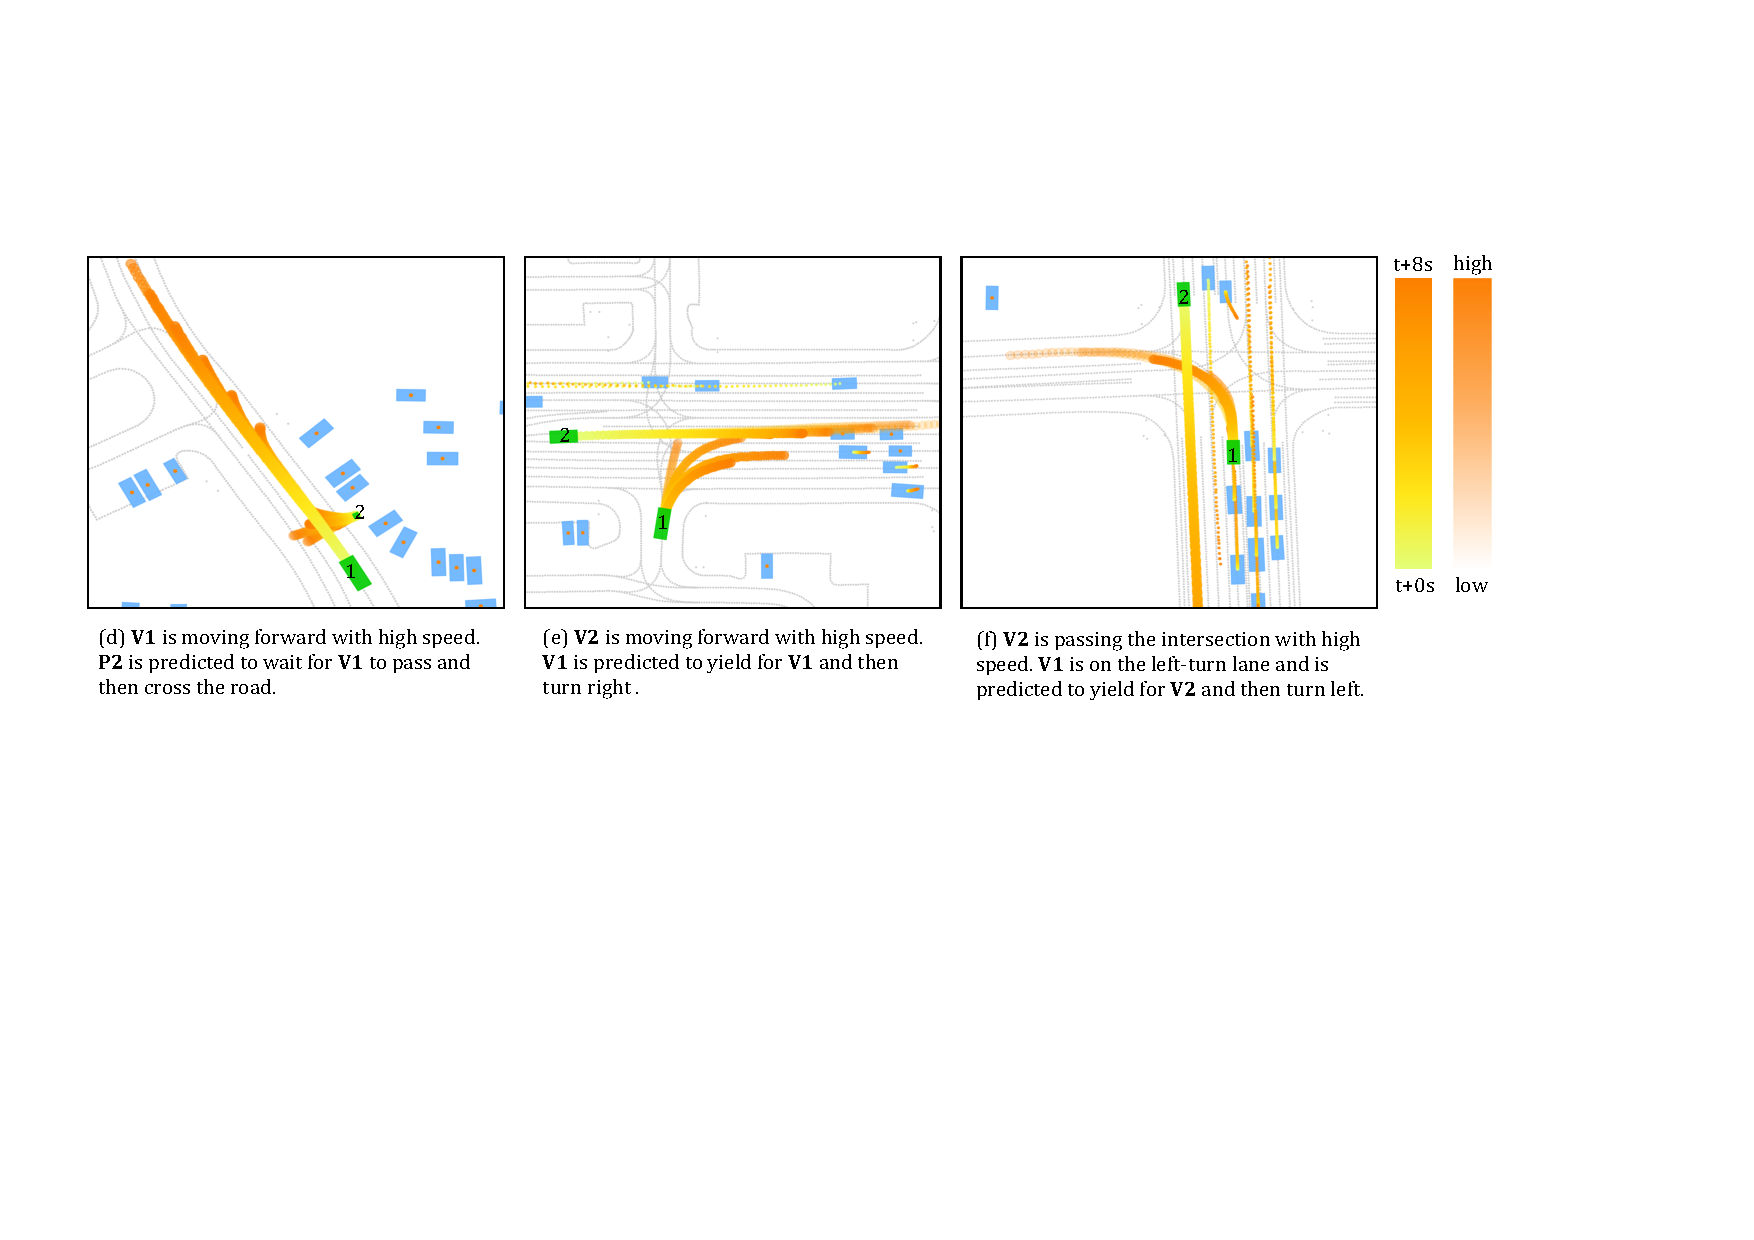
\includegraphics[width=0.99\linewidth]{figures/supp_demo_2.pdf}\\
		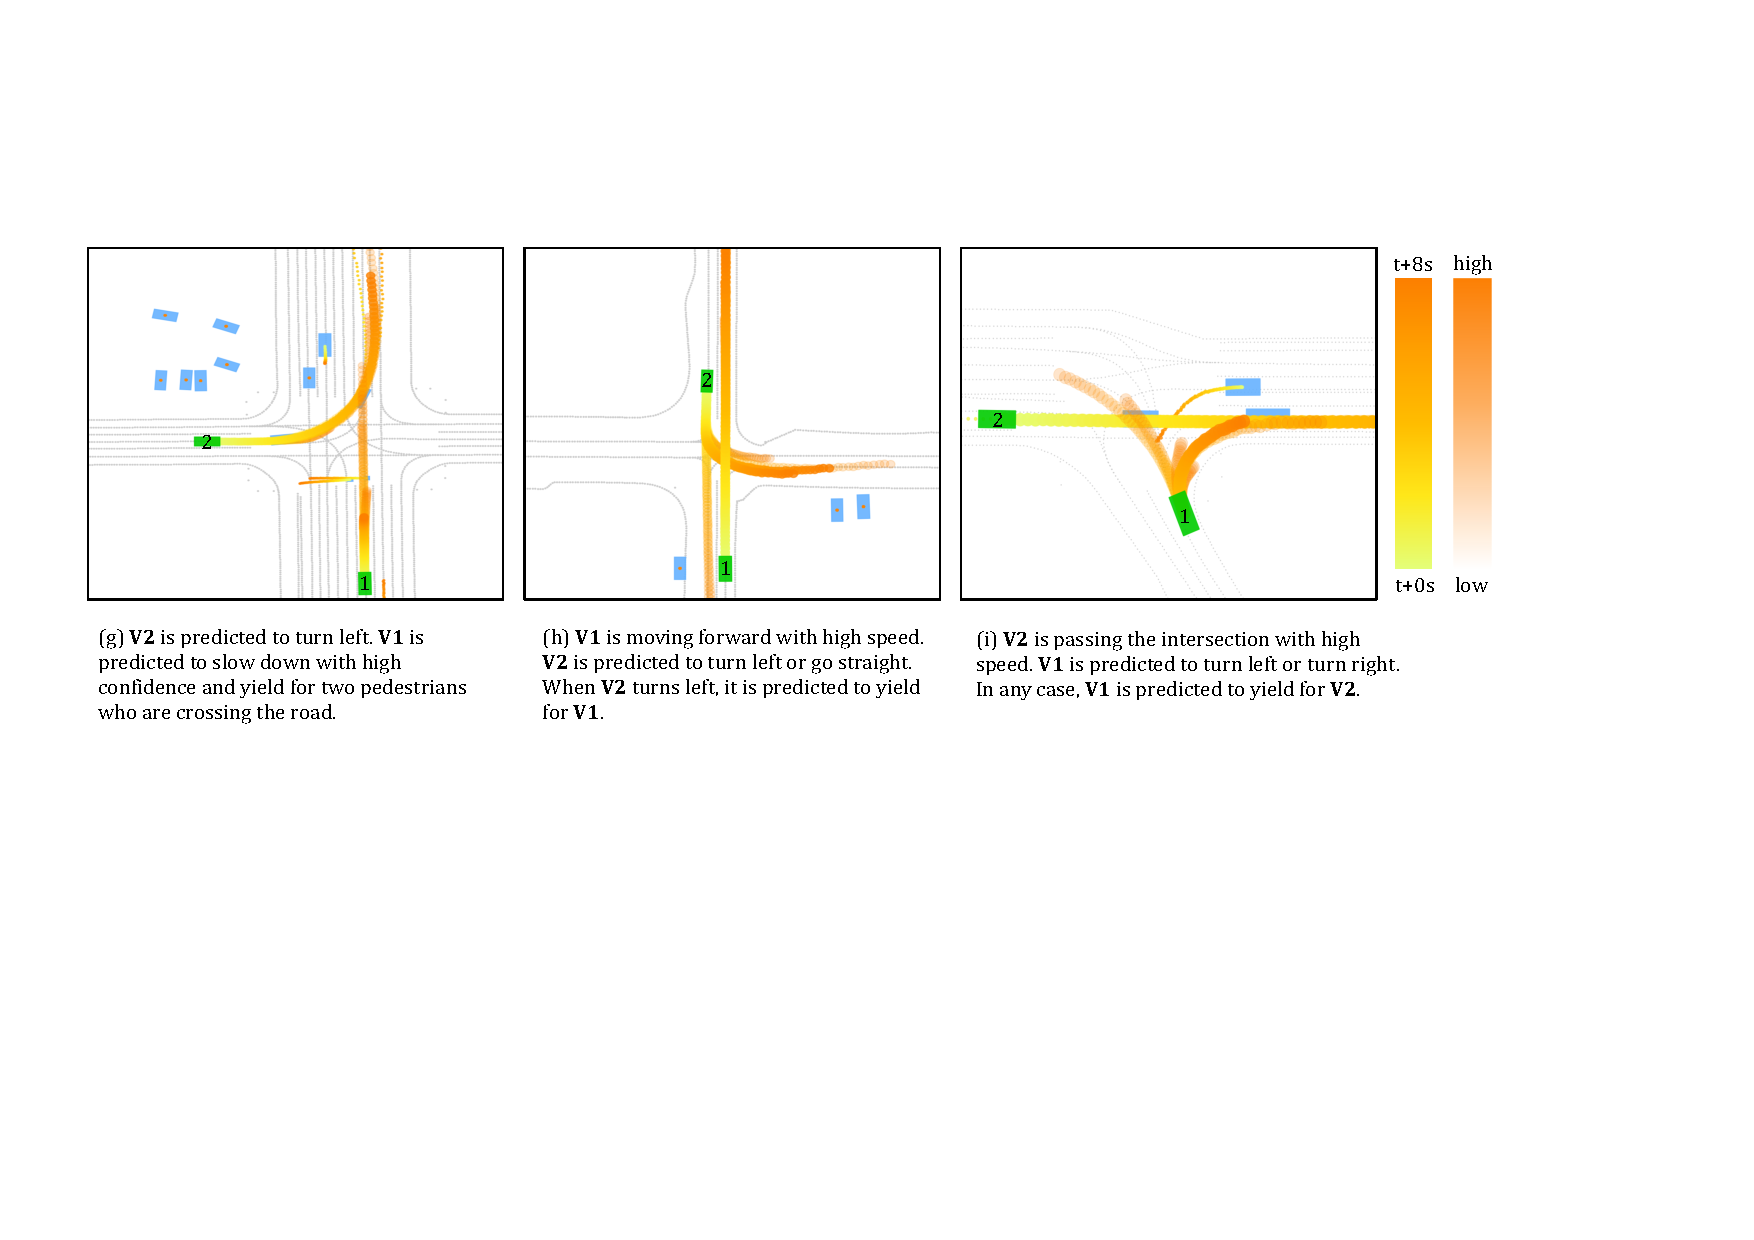
\includegraphics[width=0.99\linewidth]{figures/supp_demo_3.pdf}\\
% 		\vspace{-2mm}
		\caption{MTR框架在WOMD上的定性结果。每个场景中有两个目标智能体（绿色矩形），模型为每个目标智能体预测6条多模态未来轨迹。对其他智能体（蓝色矩形），密集未来预测模块预测单条轨迹。使用渐变色可视化不同未来时间步的轨迹路点，轨迹置信度通过不同透明度展示。缩写：车辆（V）、行人（P）。}
		\label{fig:demo_supp}
% 		\vspace{-3mm}
	\end{figure*}
    
    
   
\section{符号说明}\label{sec:notations}
如表~\ref{tab:notations_lookup}所示，提供论文中符号的对照表。

\begin{table}[h]
\caption{论文符号对照表。}
\vspace{-2mm}
\label{tab:notations_lookup}
\begin{center}
\begin{tabular}{cl}
\Xhline{2\arrayrulewidth}
% \hline 
$A_{\text{in}}$  & 智能体的输入历史运动状态 \\
$M_{\text{in}}$ & 折线表示的输入地图特征\\
$C_a$ & 智能体状态的输入特征维度 \\
$N_a$    & 智能体数量 \\
$t$ & 给定历史帧数 \\ 
$N_m$ & 地图折线数量 \\
$n$ & 每条地图折线中的点数 \\
$A_{\text{past}}$ & 折线编码器后的智能体特征 \\
$A_{\text{future}}$ & 密集预测轨迹的编码未来特征（所有智能体）\\
$A$ & Transformer编码器中的智能体特征 \\
$M$ & Transformer编码器中的地图特征 \\
$D$ & Transformer隐藏特征维度 \\
PE & 正弦位置编码函数 \\ 
$\kappa$ & k近邻算法函数 \\ 
$T$ & 待预测的未来帧数 \\
$S_i$ & 时间步$i$所有智能体的预测未来位置和速度\\
$I$ & 静态意图点 \\
$Q_I$ & 静态意图查询\\
$Q_S^{j}$ & 第$j$个解码器层中的动态搜索查询 \\
$Y^j_{1:T}$ & 第$j$个解码器层中的预测未来轨迹 \\
$L$ & 沿预测轨迹收集的地图折线数量 \\
$C^{j-1}$ & 第$j$个解码器层的输入查询内容特征 \\ 
$C^j_{\text{sa}}$ & 第$j$个解码器层自注意力后的查询内容特征 \\ 
$C^j_A$ & 第$j$个解码器层交叉注意力后的查询智能体特征 \\
$C^j_M$ & 第$j$个解码器层交叉注意力后的查询地图特征\\
$\alpha$ & 动态地图收集函数\\
$Z^j_{1:T}$ & 第$j$个解码器层中的预测GMM参数 \\ 
$p_k$ & GMM中第$k$个分量的预测概率\\ 
$\mathcal{N}_k$ & GMM中第$k$个分量的函数\\ 
$\mathcal{K}$ & 每个GMM的分量数量\\ 
$P_i^j(o)$ & 智能体在空间位置$o$和时间步$i$的预测出现概率\\ 
\Xhline{2\arrayrulewidth}
\end{tabular}
\end{center}
\end{table}
    

	
\end{document}